% This LaTeX was auto-generated from MATLAB code.
% To make changes, update the MATLAB code and export to LaTeX again.

\documentclass{article}

\usepackage[utf8]{inputenc}
\usepackage[T1]{fontenc}
\usepackage{lmodern}
\usepackage{graphicx}
\usepackage{color}
\usepackage{listings}
\usepackage{hyperref}
\usepackage{amsmath}
\usepackage{amsfonts}
\usepackage{epstopdf}
\usepackage{matlab}

\sloppy
\epstopdfsetup{outdir=./}
\graphicspath{ {./lab1live_images/} }

\begin{document}

\begin{par}
\begin{flushleft}
\textbf{Question 1} :
\end{flushleft}
\end{par}

\begin{par}
\begin{flushleft}
 Repeat this exercise with the coordinates p and q set to (5, 9), (9, 5), (17, 9), (17, 121), (5, 1) and (125, 1) respectively. What do you observe?
\end{flushleft}
\end{par}

\begin{matlabcode}
figure
fftwave(5,9)
\end{matlabcode}
\begin{center}
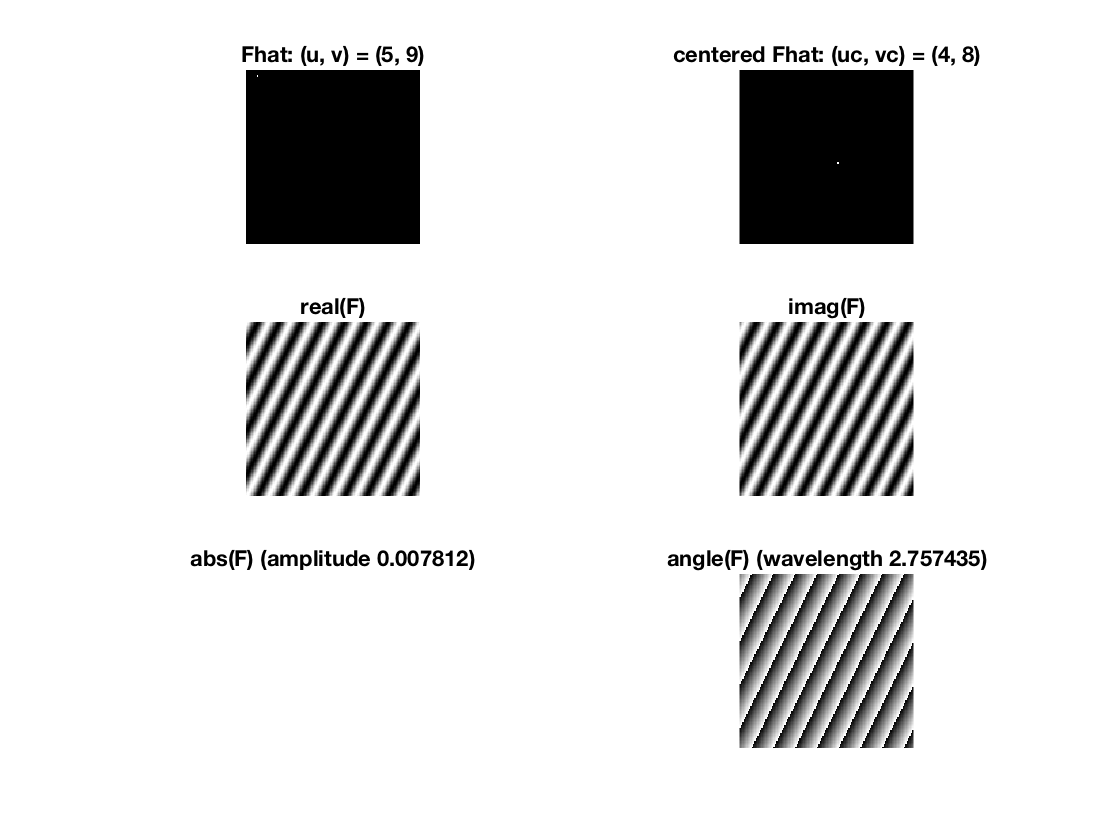
\includegraphics[width=\maxwidth{56.196688409433015em}]{figure_0}
\end{center}
\begin{matlabcode}
figure
fftwave(1,1)
\end{matlabcode}
\begin{center}
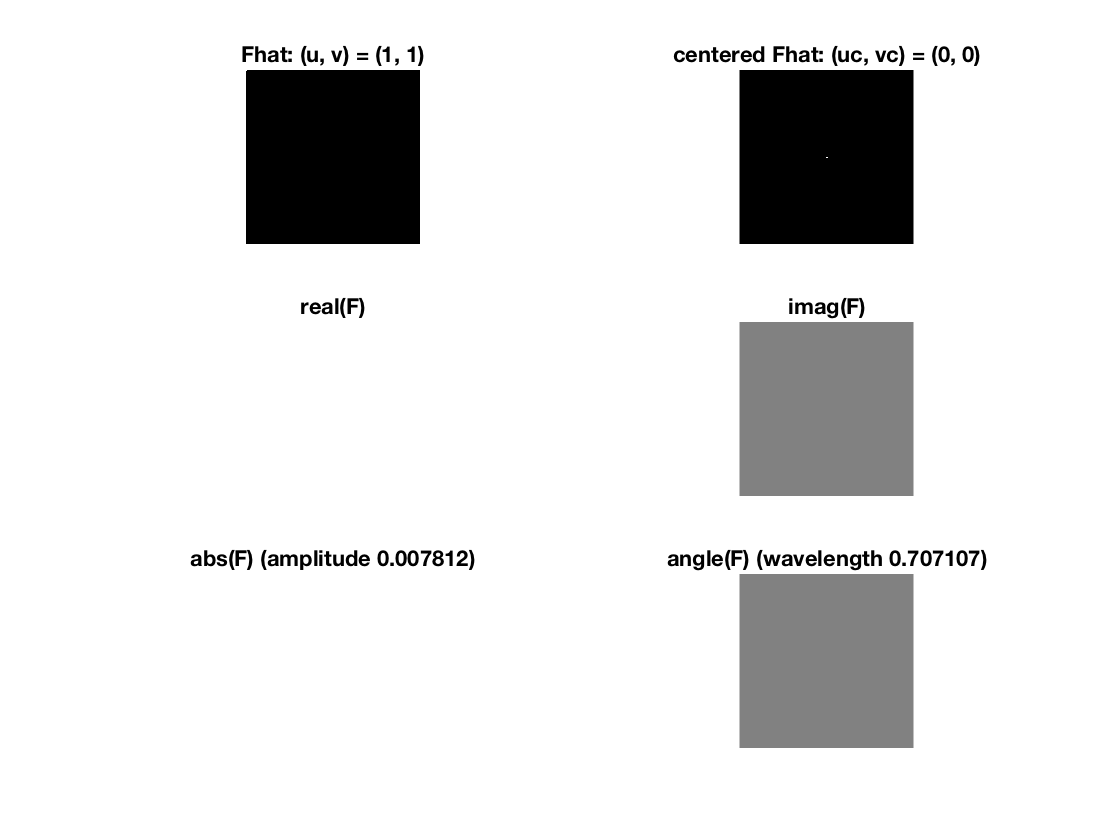
\includegraphics[width=\maxwidth{56.196688409433015em}]{figure_1}
\end{center}
\begin{matlabcode}
figure
fftwave(9,5)
\end{matlabcode}
\begin{center}
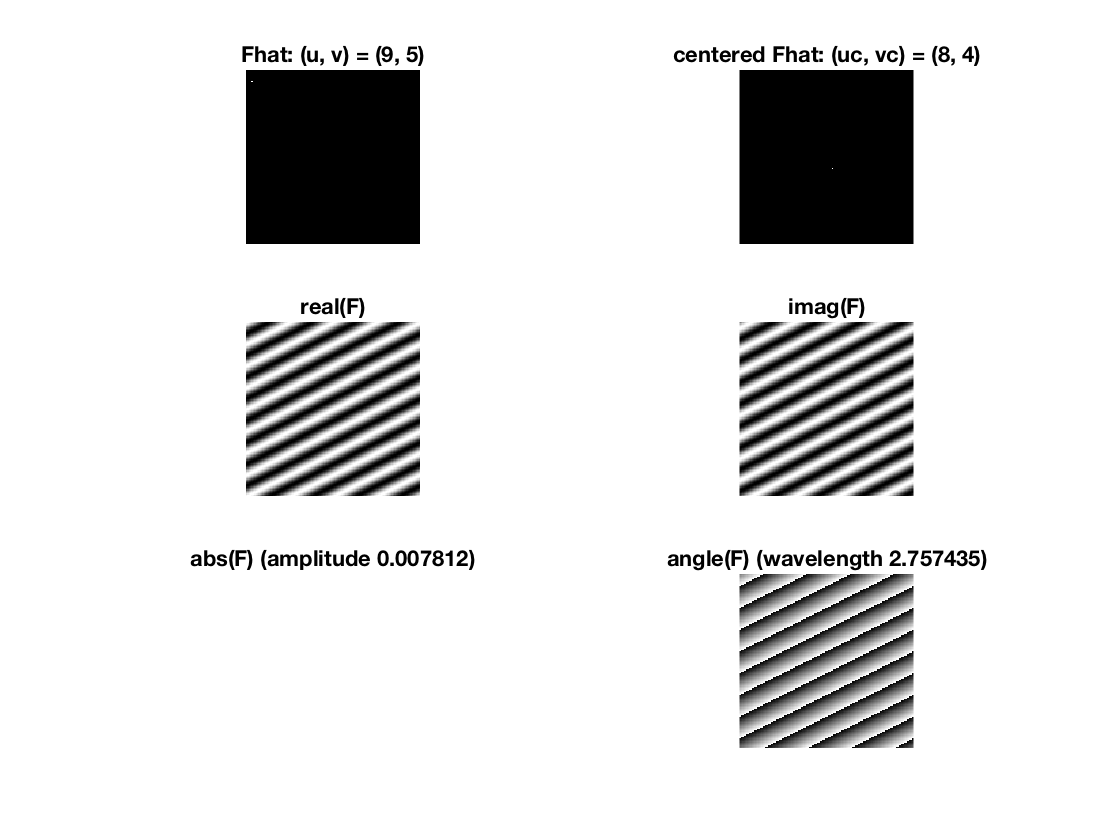
\includegraphics[width=\maxwidth{56.196688409433015em}]{figure_2}
\end{center}
\begin{matlabcode}
figure
fftwave(17,9)
\end{matlabcode}
\begin{center}
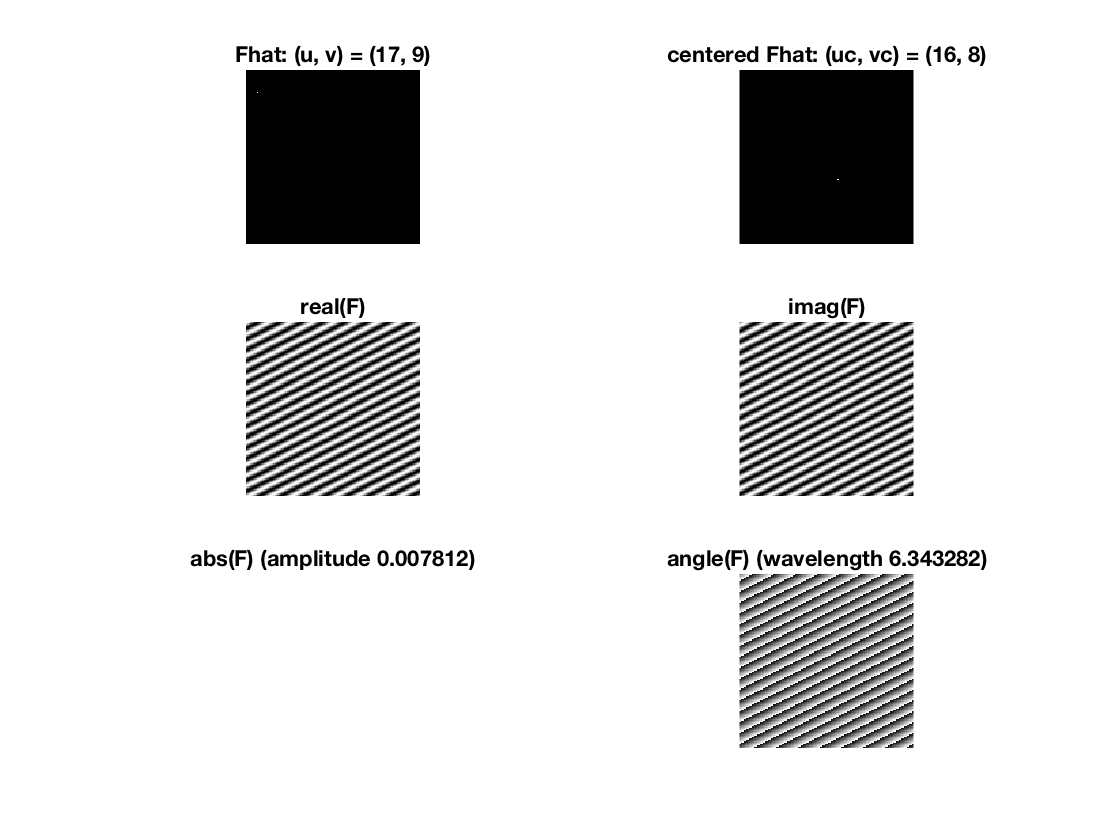
\includegraphics[width=\maxwidth{56.196688409433015em}]{figure_3}
\end{center}
\begin{matlabcode}
figure
fftwave(121,17)
\end{matlabcode}
\begin{center}
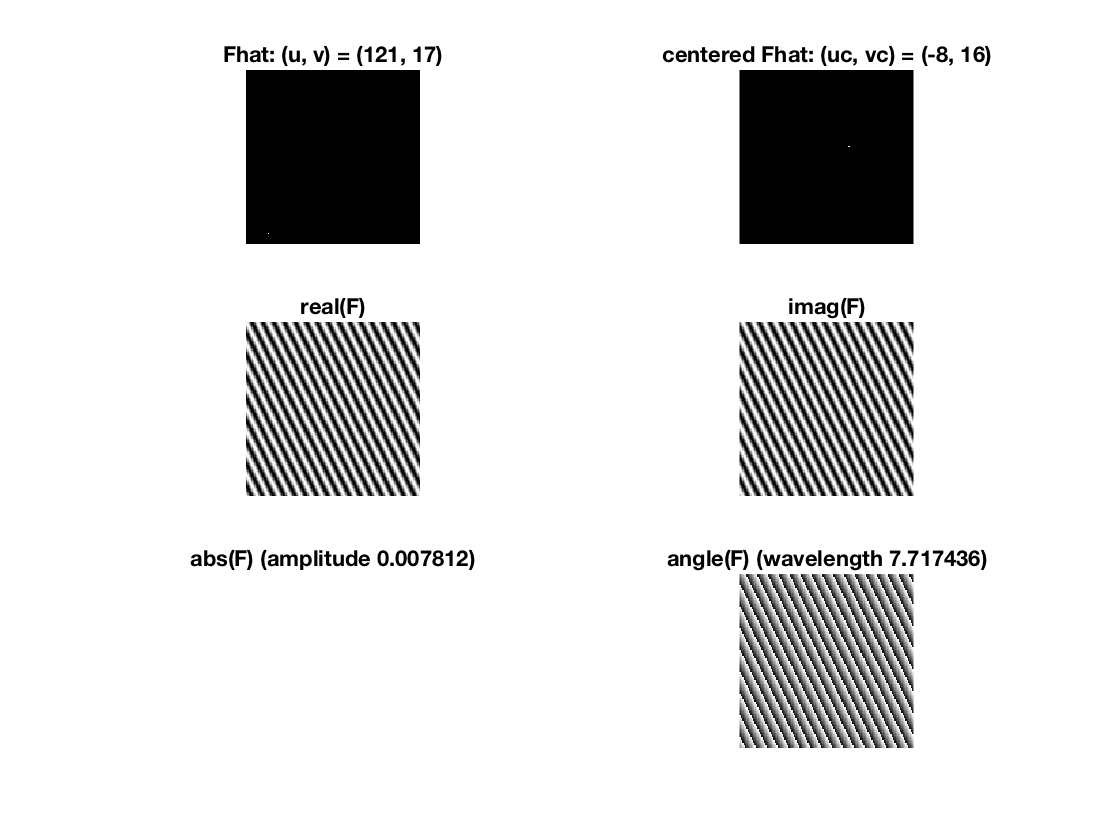
\includegraphics[width=\maxwidth{56.196688409433015em}]{figure_4}
\end{center}
\begin{matlabcode}
figure
fftwave(5,1)
\end{matlabcode}
\begin{center}
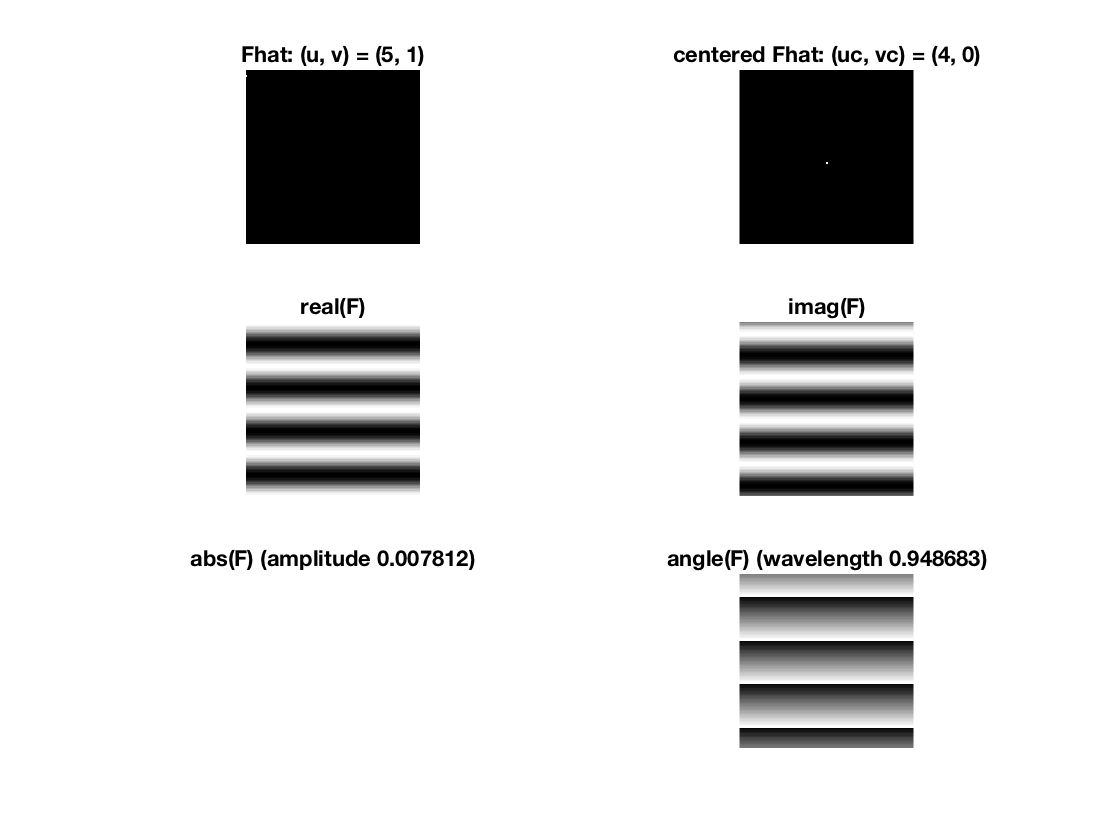
\includegraphics[width=\maxwidth{56.196688409433015em}]{figure_5}
\end{center}
\begin{matlabcode}
figure
fftwave(125,1)
\end{matlabcode}
\begin{center}
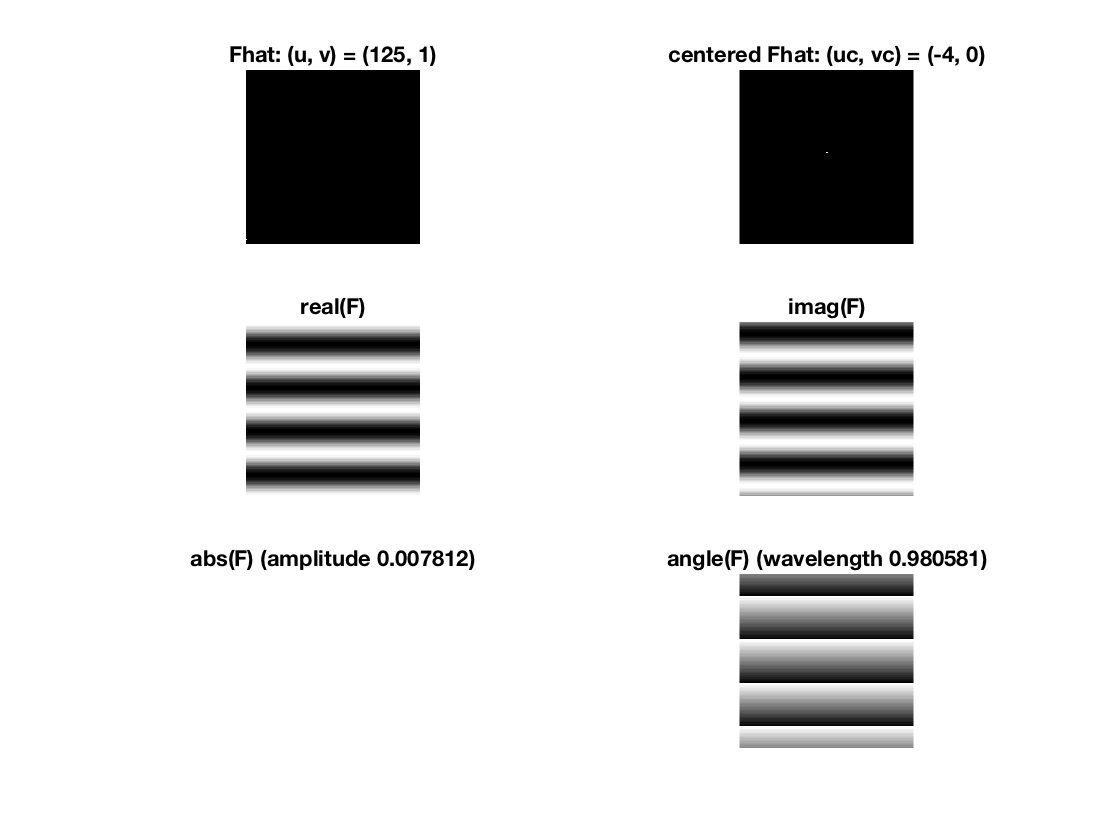
\includegraphics[width=\maxwidth{56.196688409433015em}]{figure_6}
\end{center}

\begin{par}
\begin{flushleft}
\textbf{Answers:}
\end{flushleft}
\end{par}

\begin{par}
\begin{flushleft}
the (p,q) locates more away from the center, the closer the new place when shift the (1,1) into the center (fftshift function). When p and q is less than size/2, The larger the p and q are,  the faster the frequency of the two axis, which means more strips on the figure when showing the real part and the imagine part of the image in spatial domain. When p and q is equal to the the half of size , it reaches the highest frequency and the image has no strips but instantly change of the color.(see figure 3 on question 5). When p or q is larger than the size/2, the strip become less and less.
\end{flushleft}
\end{par}


\begin{par}
\begin{flushleft}
\underline{\_\_\_\_\_\_\_\_\_\_\_\_\_\_\_\_\_\_\_\_\_\_\_\_\_\_\_\_\_\_\_\_\_\_\_\_\_\_\_\_\_\_\_\_\_\_}
\end{flushleft}
\end{par}

\begin{par}
\begin{flushleft}
\textbf{Question 2} :
\end{flushleft}
\end{par}

\begin{par}
\begin{flushleft}
Explain how a position (p, q) in the Fourier domain will be projected as a sine wave in the spatial domain. Illustrate with a Matlab figure.
\end{flushleft}
\end{par}

\begin{matlabcode}
p=5;
q=9;
Fhat = zeros(128, 128);
Fhat(p, q) = 1;
F = ifft2(Fhat);
figure
subplot(1,2,1)
Fabsmax = max(abs(F(:)));
showgrey(real(F),64,-Fabsmax, Fabsmax);
title(sprintf('real(F) on (%d,%d)',p,q))
subplot(1,2,2)
p=121;
q=17;
Fhat = zeros(128, 128);
Fhat(p, q) = 1;
F = ifft2(Fhat);
Fabsmax = max(abs(F(:)));
showgrey(real(F),64,-Fabsmax, Fabsmax);
title(sprintf('real(F) on (%d,%d)',p,q))
\end{matlabcode}
\begin{center}
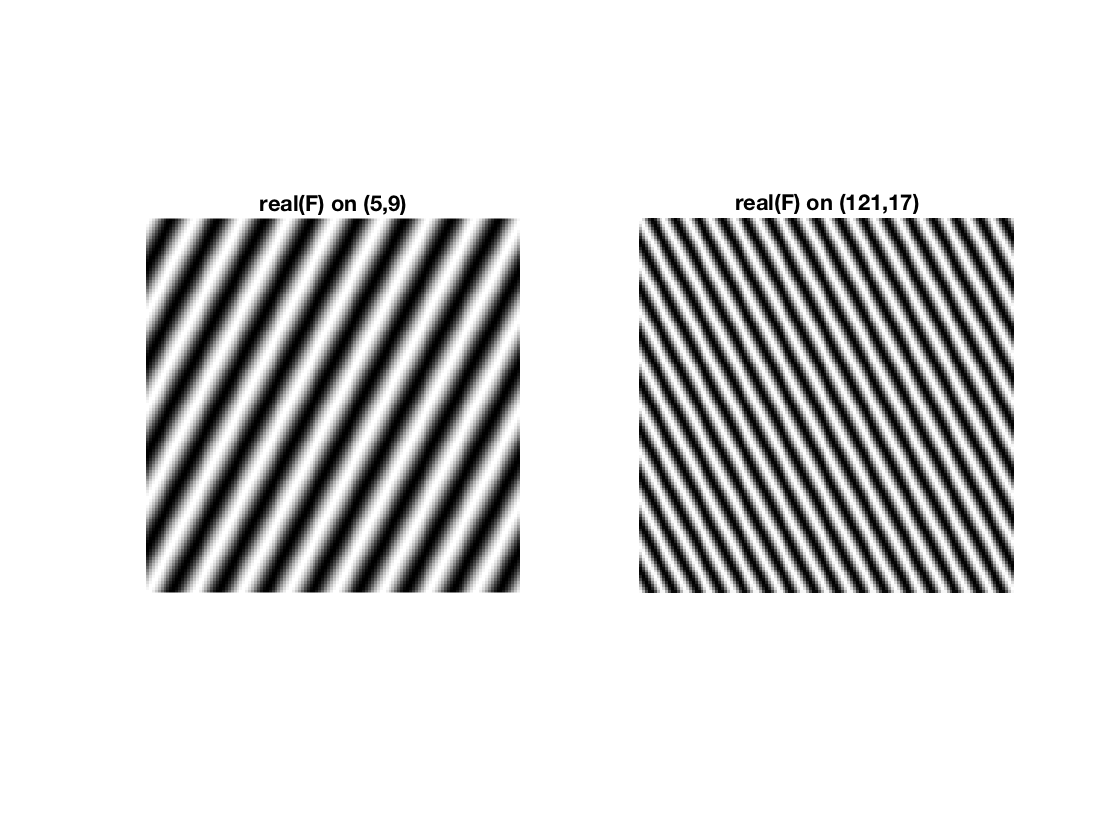
\includegraphics[width=\maxwidth{56.196688409433015em}]{figure_7}
\end{center}

\begin{par}
\begin{flushleft}
\textbf{Answer:}
\end{flushleft}
\end{par}

\begin{par}
\begin{flushleft}
Figure 1 and 2 shows the example position of(p,q) = (5,9) (right) and  (p,q) =(121,17) (left). From Figure 1 and Figure2 we know that the direction of the sine wave point to the center when we do \textit{fftshift.} 
\end{flushleft}
\end{par}


\begin{par}
\begin{flushleft}
\_\_\_\_\_\_\_\_\_\_\_\_\_\_\_\_\_\_\_\_\_\_\_\_\_\_\_\_\_\_\_\_\_\_\_\_\_\_\_\_\_\_\_\_\_\_
\end{flushleft}
\end{par}

\begin{par}
\begin{flushleft}
\textbf{Question 3 }:
\end{flushleft}
\end{par}

\begin{par}
\begin{flushleft}
How large is the amplitude? Write down the expression derived from Equation (4) in the notes. Complement the code (variable amplitude) accordingly.
\end{flushleft}
\end{par}

\begin{par}
\begin{flushleft}
\textbf{Answer:}
\end{flushleft}
\end{par}

\begin{par}
\begin{flushleft}
First of all, we do the inverse Fourier transform on :
\end{flushleft}
\end{par}

\begin{par}
$$f\left(m,n\right)=\frac{1}{\mathrm{MN}}\sum_{u=0}^{127} \sum_{v=0}^{127} F\left(u,v\right)e^{\mathrm{i2}\pi \left(\frac{\mathrm{mu}}{M}+\frac{\mathrm{nv}}{\text{ }N}\right)}$$
\end{par}

\begin{par}
\begin{flushleft}
Where M and N is 128 in our case and  equals 1 only when (u,v) = (p,q), otherwise equals 0. Therefore we know that f(m,n) equals :
\end{flushleft}
\end{par}

\begin{par}
$$f\left(m,n\right)=\frac{1}{{128}^2 }e^{-i2\pi \left(\frac{\mathrm{pm}}{M}+\frac{\mathrm{qn}}{N}\right)}$$
\end{par}

\begin{par}
\begin{flushleft}
Therefore we know that the amplitude is $\frac{1}{{128}^2 }$.
\end{flushleft}
\end{par}


\begin{par}
\begin{flushleft}
\_\_\_\_\_\_\_\_\_\_\_\_\_\_\_\_\_\_\_\_\_\_\_\_\_\_\_\_\_\_\_\_\_\_\_\_\_\_\_\_\_\_\_\_\_\_
\end{flushleft}
\end{par}

\begin{par}
\begin{flushleft}
\textbf{Question 4}:
\end{flushleft}
\end{par}

\begin{par}
\begin{flushleft}
How does the direction and length of the sine wave depend on p and q? Write down the explicit expression that can be found in the lecture notes. Complement the code (variable wavelength) accordingly.
\end{flushleft}
\end{par}

\begin{par}
\begin{flushleft}
\textbf{Answer:}
\end{flushleft}
\end{par}

\begin{par}
\begin{flushleft}
The wavelength of the sin wave is $\lambda =\frac{1}{\sqrt{u^2 +v^2 }}$, where u and v are the frequencies along r and c. In our case, by observation, we found that the frequency $u=\frac{1}{\mathrm{uc}-1}$ and frequency $v=\frac{1}{\mathrm{vc}-1}$,Therefore, the wavelength of the sine wave is
\end{flushleft}
\end{par}

\begin{par}
\begin{center}
 $\lambda =\frac{1}{\sqrt{\frac{1}{{\left(\mathrm{uc}-1\right)}^2 }+\frac{1}{{\left(\mathrm{vc}-1\right)}^2 }}}$,
\end{center}
\end{par}

\begin{par}
\begin{flushleft}
As for the direction of the sine wave, it is the diagonal of the image that point to where the center is on frequency domain.
\end{flushleft}
\end{par}


\begin{par}
\begin{flushleft}
\_\_\_\_\_\_\_\_\_\_\_\_\_\_\_\_\_\_\_\_\_\_\_\_\_\_\_\_\_\_\_\_\_\_\_\_\_\_\_\_\_\_\_\_\_\_
\end{flushleft}
\end{par}

\begin{par}
\begin{flushleft}
\textbf{Question 5:}
\end{flushleft}
\end{par}

\begin{par}
\begin{flushleft}
What happens when we pass the point in the center and either p or q exceeds half the image size? Explain and illustrate graphically with Matlab!
\end{flushleft}
\end{par}

\begin{par}
\begin{flushleft}
\textbf{Answer}:
\end{flushleft}
\end{par}

\begin{matlabcode}
figure
fftwave(64,64)
\end{matlabcode}
\begin{center}
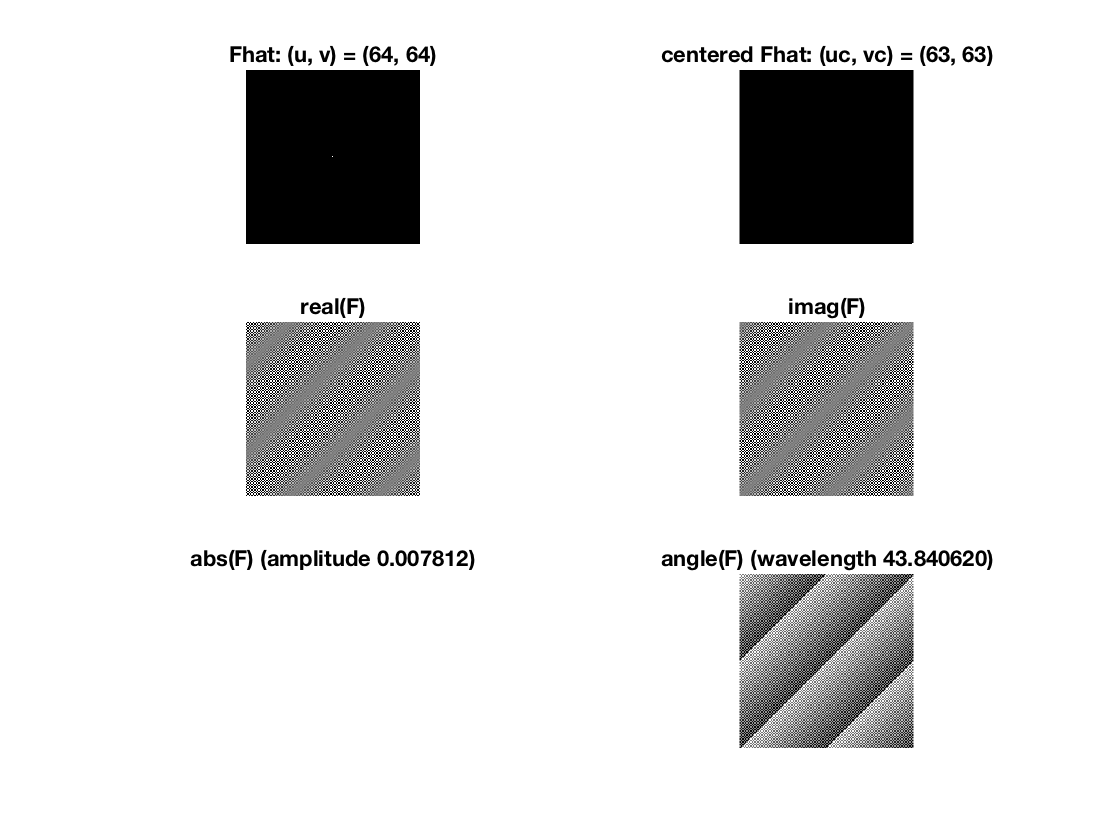
\includegraphics[width=\maxwidth{56.196688409433015em}]{figure_8}
\end{center}

\begin{par}
\begin{flushleft}
Figure 3 shows the real part of the frequency when (p , q) is \textit{(65,65)}. From figure 3 we knows that the frequency of both side are maximum, where there is no clear strips on it .
\end{flushleft}
\end{par}

\begin{par}
\begin{flushleft}
When we zoom in and see, we can see that it is looks like the figure below:
\end{flushleft}
\end{par}

\begin{par}
\begin{flushleft}
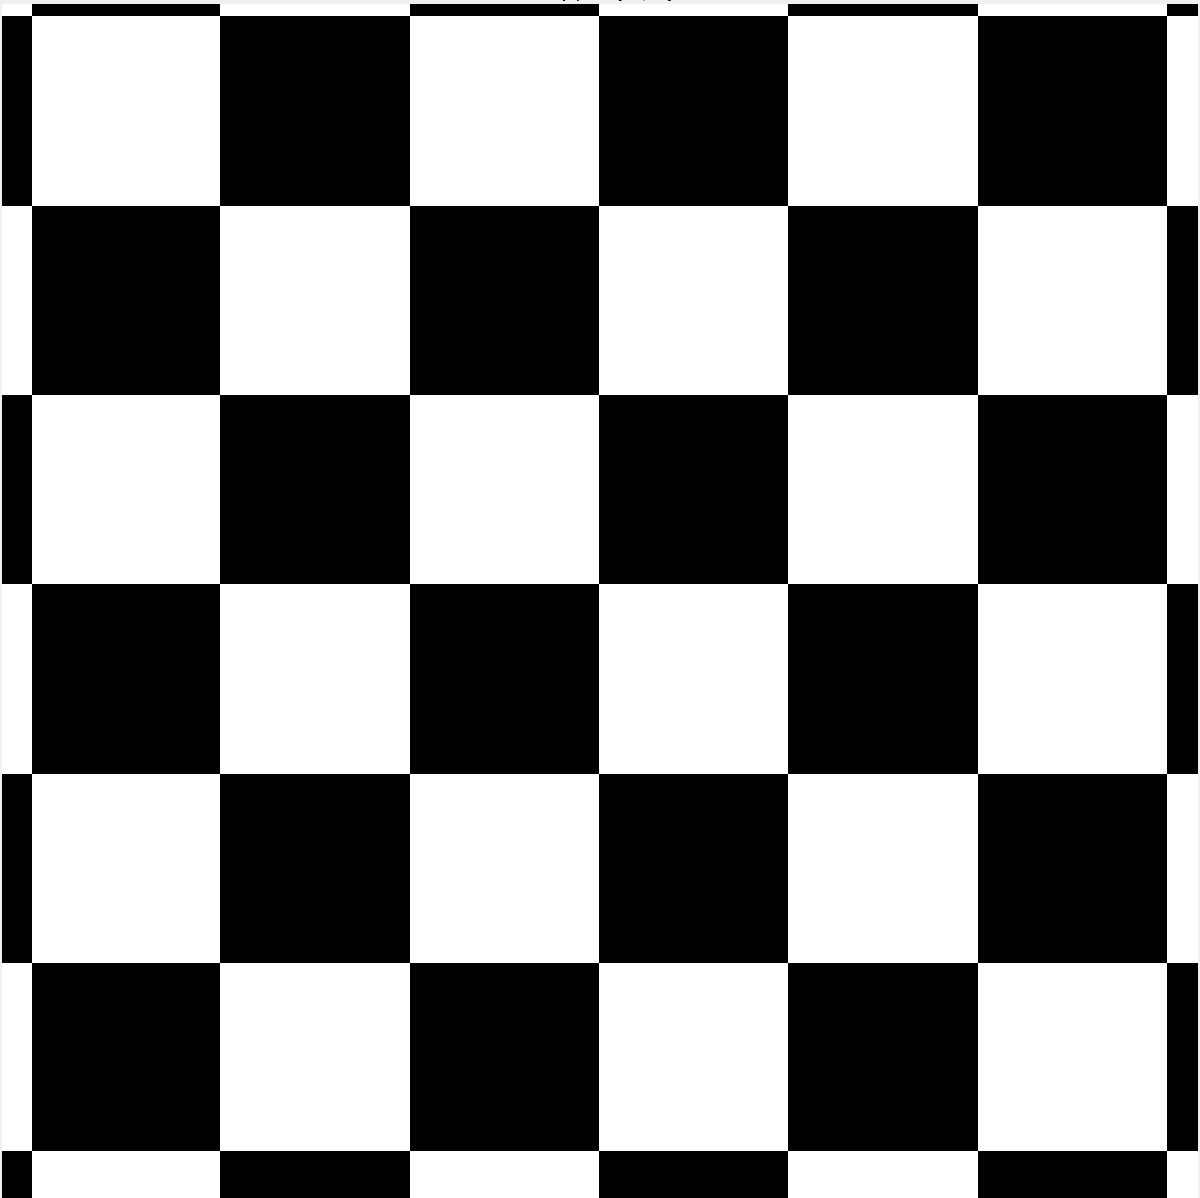
\includegraphics[width=\maxwidth{18.564977420973406em}]{image_0}
\end{flushleft}
\end{par}

\begin{par}
\begin{flushleft}
After we exceed \textit{(65,65)}, we can see that the frequency on sine wave will gradually reduce and is the same as the frequency in the point \textit{(P}\textit{1, }\textit{q}\textit{1}\textit{)},
\end{flushleft}
\end{par}

\begin{par}
\begin{flushleft}
Where \textit{|P - 1 - size | = P}\textit{1}\textit{-1}  and  \textit{|q - 1 - size | = q}\textit{1}\textit{-1}, while P1 and q1 do not exceed half of the image.
\end{flushleft}
\end{par}


\begin{par}
\begin{flushleft}
\_\_\_\_\_\_\_\_\_\_\_\_\_\_\_\_\_\_\_\_\_\_\_\_\_\_\_\_\_\_\_\_\_\_\_\_\_\_\_\_\_\_\_\_\_\_
\end{flushleft}
\end{par}

\begin{par}
\begin{flushleft}
\textbf{Question 6 :}
\end{flushleft}
\end{par}

\begin{par}
\begin{flushleft}
What is the purpose of the instructions following the question \textit{What is done by these instructions?} in the code?
\end{flushleft}
\end{par}

\begin{par}
\begin{flushleft}
\textbf{Answer:}
\end{flushleft}
\end{par}

\begin{par}
\begin{flushleft}
It finds the new (p , q) in the coordinate system in frequency domain where (1,1) in frequency domain is shift to the middle. (this is the same as the \textit{fftshift}).
\end{flushleft}
\end{par}


\begin{par}
\begin{flushleft}
\_\_\_\_\_\_\_\_\_\_\_\_\_\_\_\_\_\_\_\_\_\_\_\_\_\_\_\_\_\_\_\_\_\_\_\_\_\_\_\_\_\_\_\_\_\_
\end{flushleft}
\end{par}

\begin{par}
\begin{flushleft}
\textbf{Question 7 }:
\end{flushleft}
\end{par}

\begin{par}
\begin{flushleft}
Why are these Fourier spectra concentrated to the borders of the images? Can you give a mathematical interpretation? Hint: think of the frequencies in the source image and consider the resulting image as a Fourier transform applied to a 2D function. It might be easier to analyze each dimension separately!
\end{flushleft}
\end{par}

\begin{par}
\begin{flushleft}
\textbf{Answer:}
\end{flushleft}
\end{par}

\begin{matlabcode}
F = [zeros(56, 128); ones(16, 128); zeros(56, 128)];
G = F';
H = F + 2 * G;
Fhat = fft2(F);
Ghat = fft2(G);
Hhat = fft2(H);

figure
subplot(3,2,1);
showgrey(F);
title('F');

subplot(3,2,3);
showgrey(G);
title('G');

subplot(3,2,5);
showgrey(H);
title('F+2G');

subplot(3,2,2);
showgrey(log(1 + abs(Fhat)));
%showgrey(log(1 + abs(fftshift(Fhat))));
title('Fhat');

subplot(3,2,4);
showgrey(log(1 + abs(Ghat)));
%showgrey(log(1 + abs(fftshift(Ghat))));
title('Ghat');

subplot(3,2,6);
showgrey(log(1 + abs(Hhat)));
%showgrey(log(1 + abs(fftshift(Hhat))));
title('Hhat');
\end{matlabcode}
\begin{center}
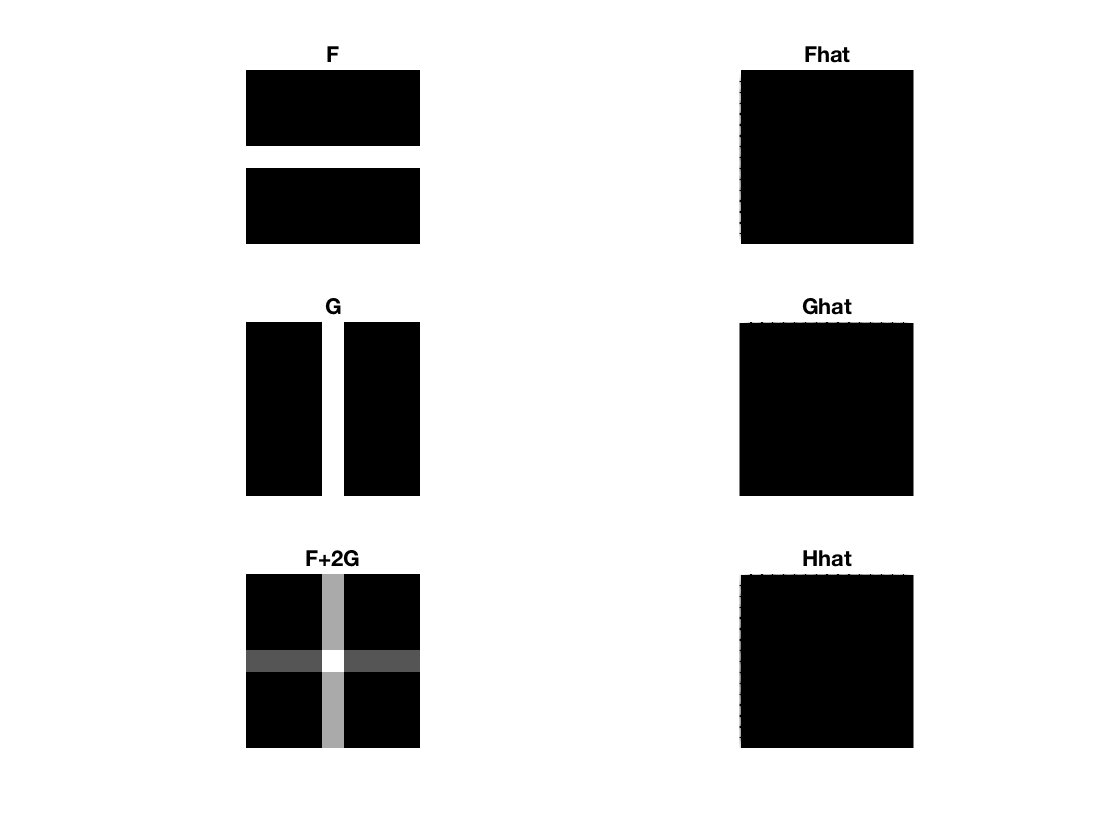
\includegraphics[width=\maxwidth{56.196688409433015em}]{figure_9}
\end{center}

\begin{par}
\begin{flushleft}
When we plot F, we know that the frequency along x (horizontal)  is 0 while the frequency along y (vertical) is 1. So when we see the plot from x axis, we can not see any sine wave but the magnitude of sine wave on y (which is 1 only). Therefore, when plotting the frequency domain of F, x is always 1 while there is a sine wave along y. which locates in the margin where x = 1.
\end{flushleft}
\end{par}

\begin{par}
\begin{flushleft}
            
\end{flushleft}
\end{par}

\begin{par}
\begin{flushleft}
When we plot G, on the other hand, the frequency along (horizontal) is 1 and the frequency along y (vertical) is 0.  When plotting the frequency domain of G, y is always 1 while there is a sine wave along x, which locates in the margin where y = 1.
\end{flushleft}
\end{par}


\begin{par}
\begin{flushleft}
\_\_\_\_\_\_\_\_\_\_\_\_\_\_\_\_\_\_\_\_\_\_\_\_\_\_\_\_\_\_\_\_\_\_\_\_\_\_\_\_\_\_\_\_\_\_
\end{flushleft}
\end{par}

\begin{par}
\begin{flushleft}
\textbf{Question 8 :}
\end{flushleft}
\end{par}

\begin{par}
\begin{flushleft}
Why is the logarithm function applied?
\end{flushleft}
\end{par}

\begin{par}
\begin{flushleft}
\textbf{Answer:}
\end{flushleft}
\end{par}

\begin{par}
\begin{flushleft}
The logarithm function can compress the dynamic range of images with large variations in pixel values and it scales this with new linearly range and displaying the spectrum.
\end{flushleft}
\end{par}


\begin{par}
\begin{flushleft}
\_\_\_\_\_\_\_\_\_\_\_\_\_\_\_\_\_\_\_\_\_\_\_\_\_\_\_\_\_\_\_\_\_\_\_\_\_\_\_\_\_\_\_\_\_\_
\end{flushleft}
\end{par}

\begin{par}
\begin{flushleft}
\textbf{Question 9 :}
\end{flushleft}
\end{par}

\begin{par}
\begin{flushleft}
What conclusions can be drawn regarding linearity? From your observations can you derive a mathematical expression in the general case?
\end{flushleft}
\end{par}

\begin{par}
\begin{flushleft}
\textbf{Answer:}
\end{flushleft}
\end{par}

\begin{par}
\begin{flushleft}
From compare F and G both in spatial and frequency domain with H, which is a linear combination of F and G, we can conclude that, first of all, when we combine two images, the new image’s Fourier transform is also the combination of the two image’s Fourier transform. This is the property of linearity. Secondly, when doing 2D discrete Fourier transform, the transform is implemented as a series of 1D Fourier transforms along each column, followed by 1D Fourier transforms along each row.
\end{flushleft}
\end{par}

\begin{par}
\begin{flushleft}
The mathematical expression is shown below:
\end{flushleft}
\end{par}

\begin{par}
\begin{flushleft}
For linearity:
\end{flushleft}
\end{par}

\begin{par}
$$F\left(a\left(f\left(m,n\right)\right)+b\left(g\left(m,n\right)\right)\right)=a\left(F\left(f\left(m,n\right)\right)\right)+b\left(F\left(f\left(m,n\right)\right)\right)$$
\end{par}

\begin{par}
\begin{flushleft}
For 2D discrete Fourier transform:
\end{flushleft}
\end{par}

\begin{par}
$$F\left(u,v\right)=\frac{1}{\sqrt{M}}\sum_{m=0}^{M-1} \left(\frac{1}{\sqrt{N}}\sum_{n=0}^{N-1} f\left(m,n\right)e^{-\mathrm{i2}\pi \left(\frac{\mathrm{nv}}{N}\right)} \right)e^{-\mathrm{i2}\pi \left(\frac{\mathrm{mu}}{M}\right)}$$
\end{par}


\begin{par}
\begin{flushleft}
\_\_\_\_\_\_\_\_\_\_\_\_\_\_\_\_\_\_\_\_\_\_\_\_\_\_\_\_\_\_\_\_\_\_\_\_\_\_\_\_\_\_\_\_\_\_
\end{flushleft}
\end{par}

\begin{par}
\begin{flushleft}
\textbf{Question 10} :
\end{flushleft}
\end{par}

\begin{par}
\begin{flushleft}
Are there any other ways to compute the last image? Remember what multiplication in Fourier domain equals to in the spatial domain! Perform these alternative computations in practice.
\end{flushleft}
\end{par}

\begin{matlabcode}
figure
showgrey(F .* G);
\end{matlabcode}
\begin{center}
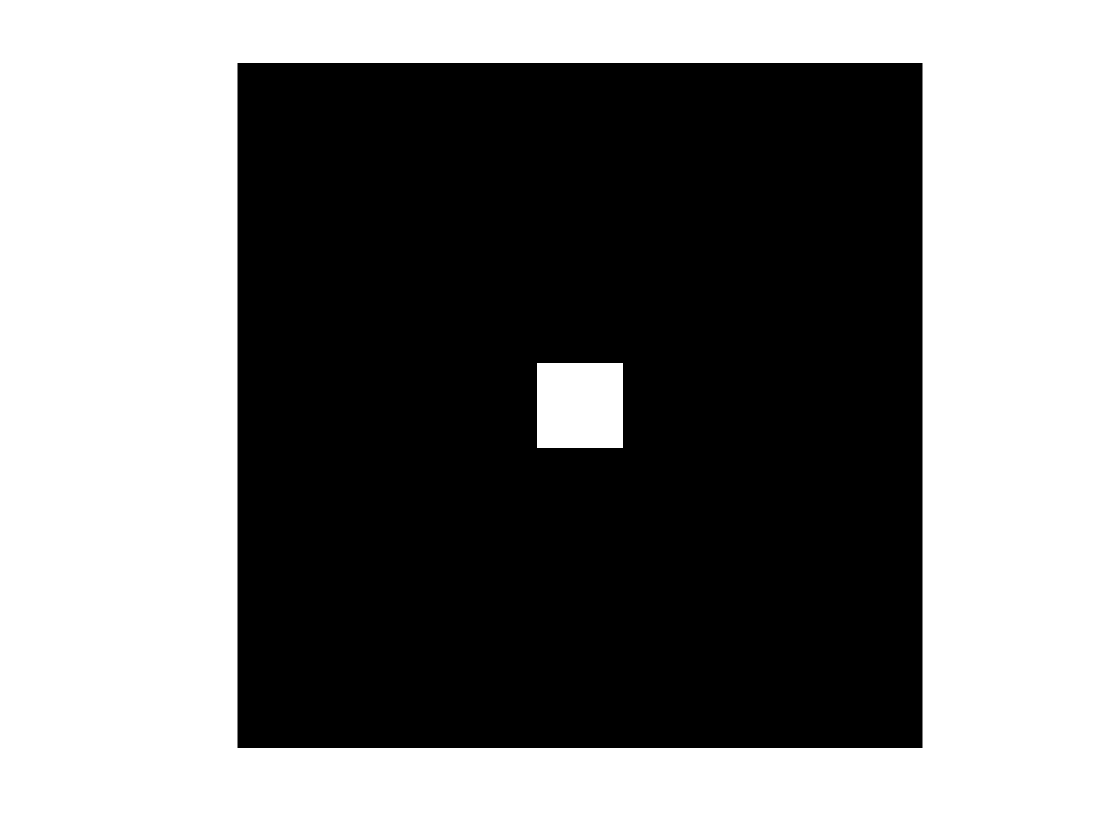
\includegraphics[width=\maxwidth{56.196688409433015em}]{figure_10}
\end{center}
\begin{matlabcode}
figure
showfs(fft2(F .* G));
\end{matlabcode}
\begin{center}
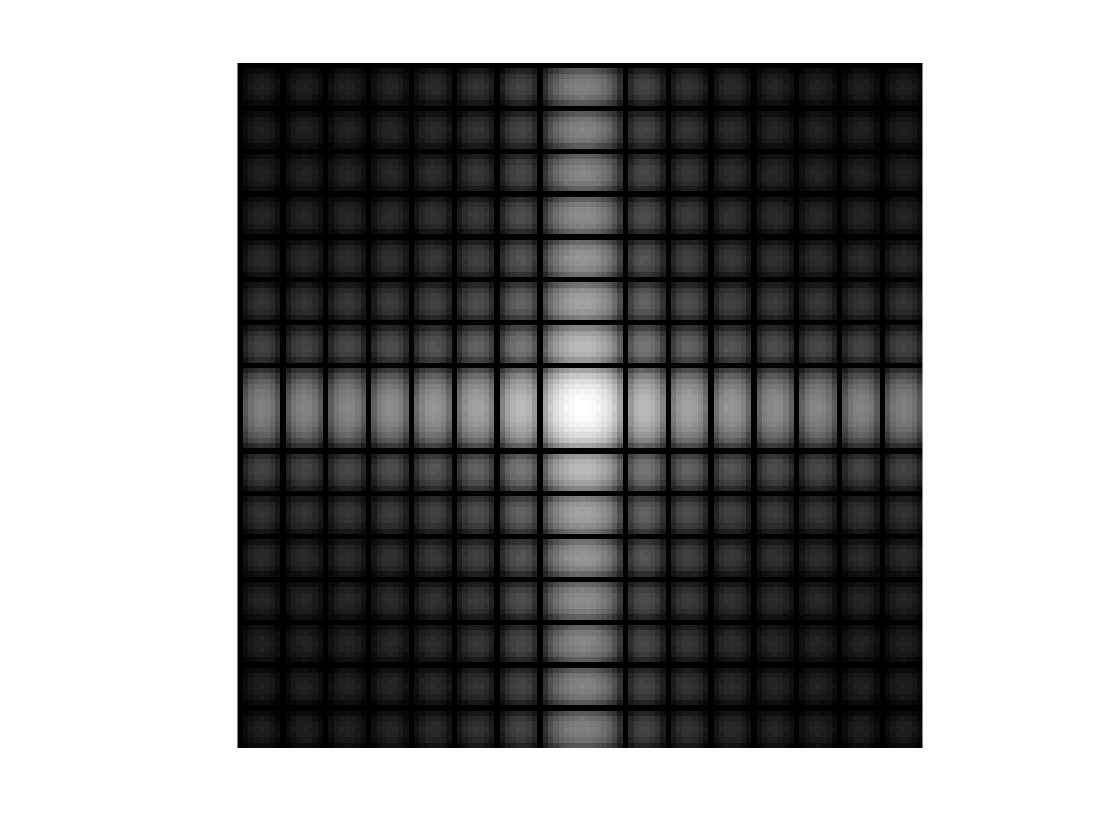
\includegraphics[width=\maxwidth{56.196688409433015em}]{figure_11}
\end{center}

\begin{par}
\begin{flushleft}
\textbf{Answer}:
\end{flushleft}
\end{par}

\begin{par}
\begin{flushleft}
Based on the convolution theorem, if we do the element-wise multiplication on spatial domain, then it is equal to do the convolution in frequency domain. Therefore, we can use following commend to find the same image :
\end{flushleft}
\end{par}

\begin{matlabcode}
figure
showfs(1/(128*128)*fftshift((conv2(fftshift(fft2(F)),fftshift(fft2(G)),'same'))));
\end{matlabcode}
\begin{center}
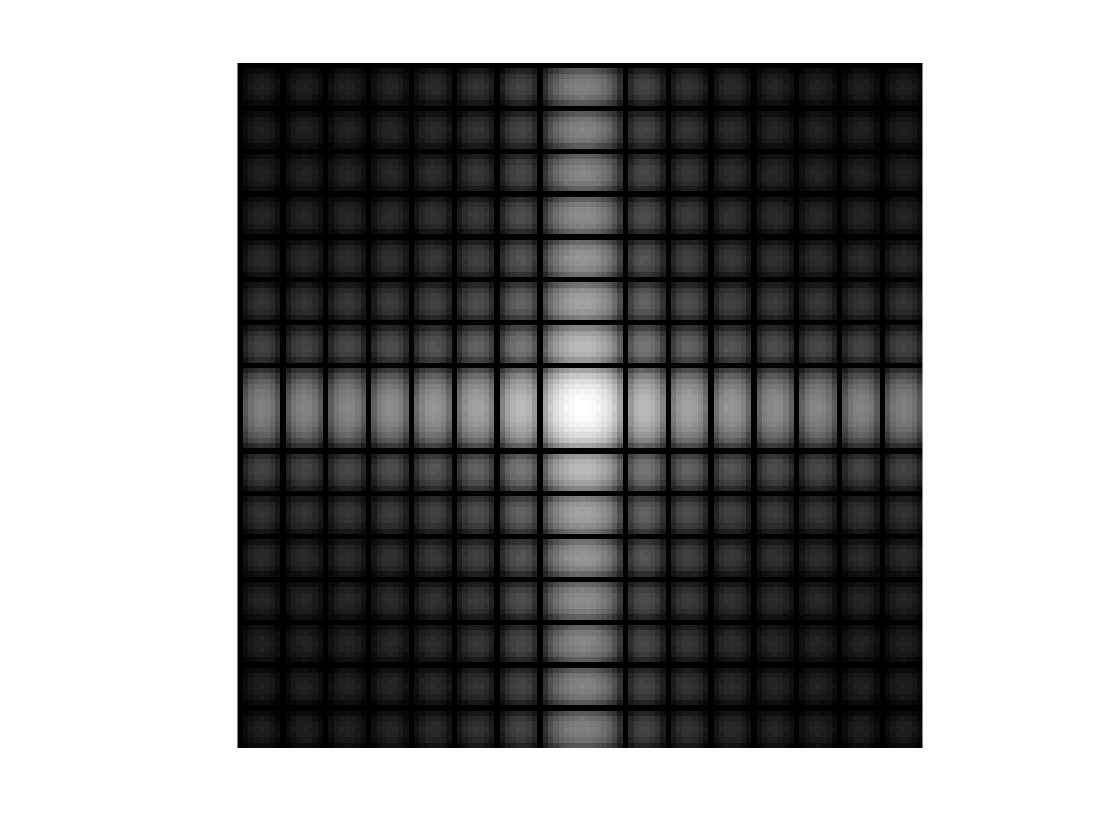
\includegraphics[width=\maxwidth{56.196688409433015em}]{figure_12}
\end{center}

\begin{par}
\begin{flushleft}
 
\end{flushleft}
\end{par}


\begin{par}
\begin{flushleft}
\_\_\_\_\_\_\_\_\_\_\_\_\_\_\_\_\_\_\_\_\_\_\_\_\_\_\_\_\_\_\_\_\_\_\_\_\_\_\_\_\_\_\_\_\_\_
\end{flushleft}
\end{par}

\begin{par}
\begin{flushleft}
\textbf{Question 11:}
\end{flushleft}
\end{par}

\begin{par}
\begin{flushleft}
What conclusions can be drawn from comparing the results with those in the previous exercise? See how the source images have changed and analyze the effects of scaling.
\end{flushleft}
\end{par}

\begin{par}
\begin{flushleft}
 
\end{flushleft}
\end{par}

\begin{matlabcode}
F_11 = [zeros(60, 128); ones(8, 128); zeros(60, 128)] .* ...
         [zeros(128, 48) ones(128, 32) zeros(128, 48)];
figure
subplot(2,2,1);
showgrey(F .* G);
title('Original image');

subplot(2,2,2);
showfs(fft2(F .* G));
title('origin image in frequency domain');

subplot(2,2,3);
showgrey(F_11);
title('compression of F');

subplot(2,2,4);
F_11hat = fft2(F_11);
showfs(F_11hat);
title('compressed image in frequency domain');
\end{matlabcode}
\begin{center}
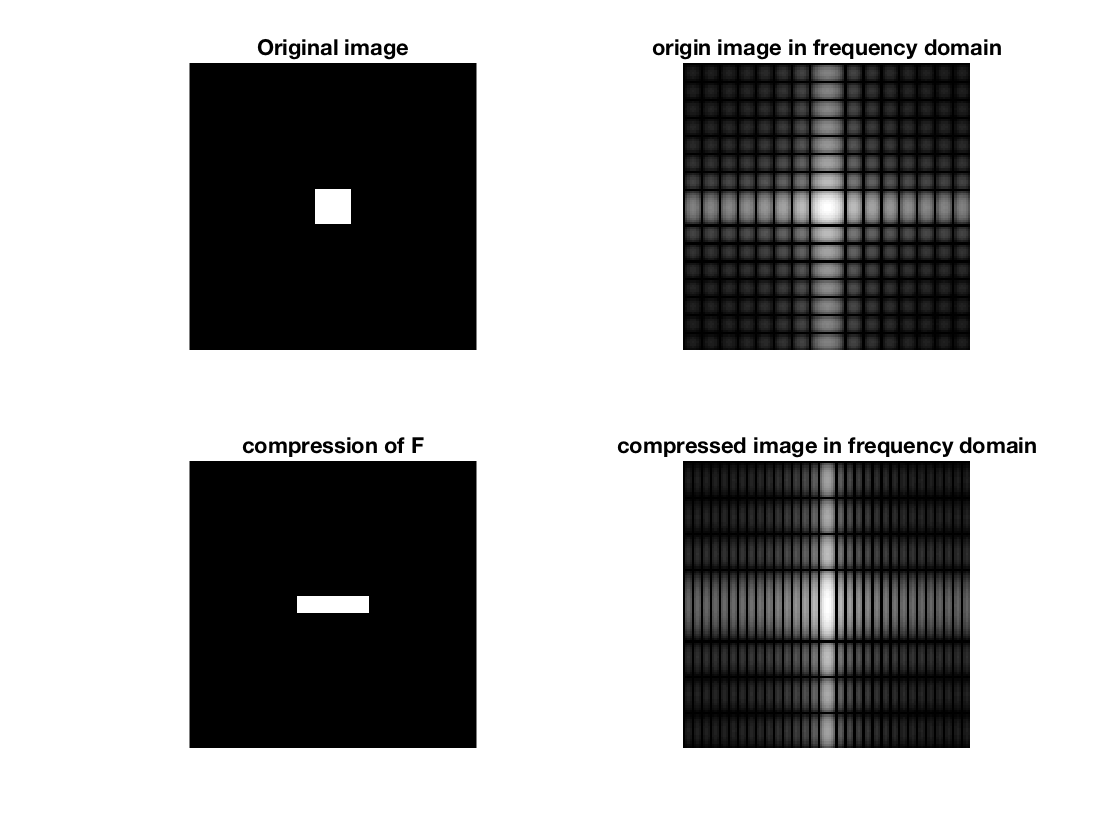
\includegraphics[width=\maxwidth{56.196688409433015em}]{figure_13}
\end{center}

\begin{par}
\begin{flushleft}
\textbf{Answers:}
\end{flushleft}
\end{par}

\begin{par}
\begin{flushleft}
            The previous image is a square in the center while the current image is a rectangle with the length is on the y-axis. In frequency domain of previous image, there is a square in the middle while in frequency domain of current image, there is a rectangle with the length on the x-axis. With the Comparison of previous image and current image, we can conclude that when there is a compression in spatial domain, there is an expansion in frequency domain. On the other hand, if there is an expansion in spatial domain, a compression occurs in frequency domain. 
\end{flushleft}
\end{par}


\begin{par}
\begin{flushleft}
\_\_\_\_\_\_\_\_\_\_\_\_\_\_\_\_\_\_\_\_\_\_\_\_\_\_\_\_\_\_\_\_\_\_\_\_\_\_\_\_\_\_\_\_\_\_
\end{flushleft}
\end{par}

\begin{par}
\begin{flushleft}
\textbf{Question 12:}
\end{flushleft}
\end{par}

\begin{par}
\begin{flushleft}
What can be said about possible similarities and differences? Hint: think of the frequencies and how they are affected by the rotation.
\end{flushleft}
\end{par}

\begin{matlabcode}
%original
figure
subplot(2,1,1);
showgrey(F_11);
title('original image of F');
subplot(2,1,2);
showfs(F_11hat);
title('frequency domain of image F');
\end{matlabcode}
\begin{center}
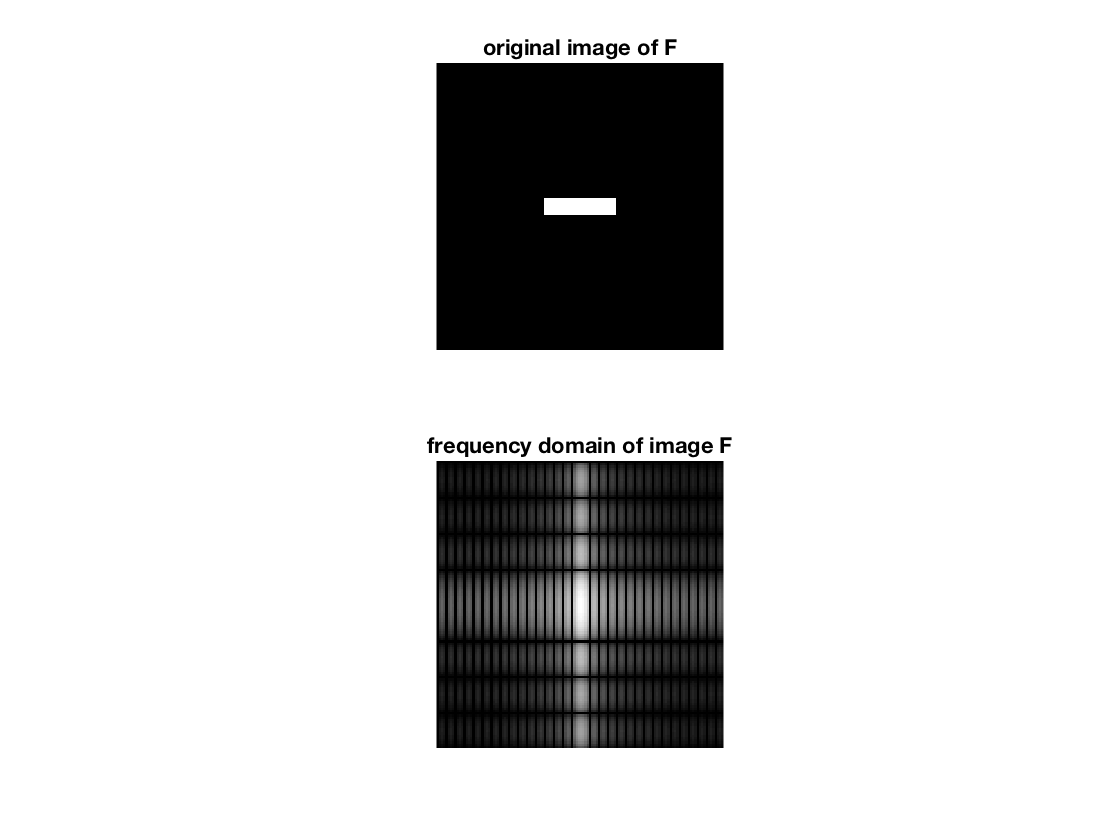
\includegraphics[width=\maxwidth{56.196688409433015em}]{figure_14}
\end{center}
\begin{matlabcode}

%rotation 
alpha = 30;
figure
G = rot(F_11, alpha); 
subplot(4,3,1);
showgrey(G)
title('rotation(a=30) of F')
subplot(4,3,2);
% figure
% axis on
Ghat = fft2(G);
showfs(Ghat);
title('rotation(a=30) of F in freq');

subplot(4,3,3);
Hhat = rot(fftshift(Ghat), -alpha);
showgrey(log(1 + abs(Hhat)))
title('rotate back(a=30) of F in freq ');

alpha = 45;
G =rot(F_11,alpha);
subplot(4,3,4);
showgrey(G)
title('rotation(a=45)of F')
subplot(4,3,5);
% figure
% axis on
Ghat = fft2(G);
showfs(Ghat);
title('rotation(a=45)of F in freq');

subplot(4,3,6);
Hhat = rot(fftshift(Ghat), -alpha);
showgrey(log(1 + abs(Hhat)))
title('rotation back(a=45)of F in freq');

alpha = 60;
G = rot(F_11,alpha);
subplot(4,3,7);
showgrey(G)
title('rotation(a=60) of F')
subplot(4,3,8);
% figure
% axis on
Ghat = fft2(G);
showfs(Ghat);
title('rotation(a=60) of F in freq');

subplot(4,3,9);
Hhat = rot(fftshift(Ghat), -alpha);
showgrey(log(1 + abs(Hhat)))
title('rotation back(a=60) of F in freq');

alpha = 90;
G = rot(F_11,alpha);
subplot(4,3,10);
showgrey(G)
title('rotation(a=90) of F')
subplot(4,3,11);
% figure
% axis on
Ghat = fft2(G);
showfs(Ghat);
title('rotation(a=90) of F in freq');

subplot(4,3,12);
Hhat = rot(fftshift(Ghat), -alpha);
showgrey(log(1 + abs(Hhat)))
title('rotation back(a=90) of F in Freq');
\end{matlabcode}
\begin{center}
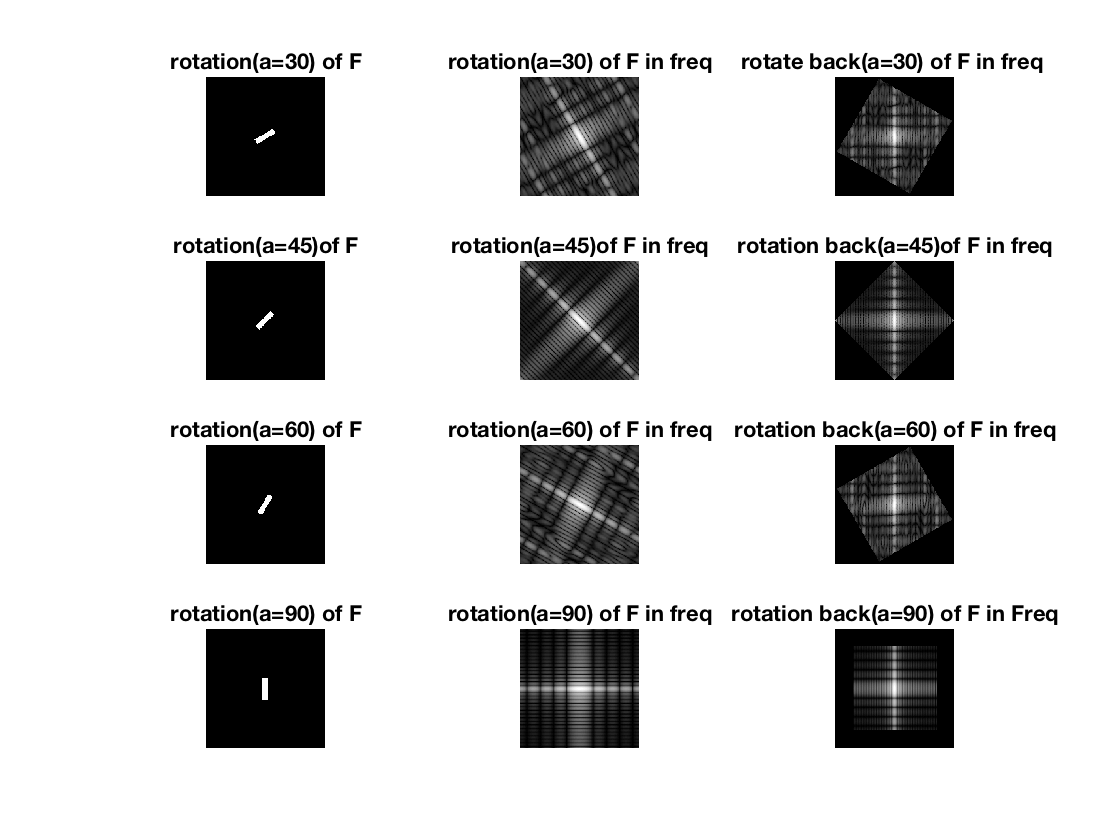
\includegraphics[width=\maxwidth{56.196688409433015em}]{figure_15}
\end{center}

\begin{par}
\begin{flushleft}
\textbf{Answer:}
\end{flushleft}
\end{par}

\begin{par}
\begin{flushleft}
When we rotate the image from spatial domain, the rotation occurs also in frequency domain with same direction and angle. However, if we rotate it back in frequency domain, some information would be shift from higher frequency to lower frequency, and we can see how many angles we rotated in the image. 
\end{flushleft}
\end{par}

\begin{par}
\begin{flushleft}
By comparing different angle rotation, we can see that only when we rotation on 45 or 90 degrees, the image of frequency doesn’t deform while when we rotation on other angles, the image of frequency deforms.
\end{flushleft}
\end{par}


\begin{par}
\begin{flushleft}
\textbf{Question 13:}
\end{flushleft}
\end{par}

\begin{par}
\begin{flushleft}
What information is contained in the phase and in the magnitude of the Fourier transform?
\end{flushleft}
\end{par}

\begin{matlabcode}
img_1 = phonecalc128;
img_2 = few128;
img_3 = nallo128;
a = 1e-10;
img_1_p2i = pow2image(img_1,a);
img_2_p2i = pow2image(img_2,a);
img_3_p2i = pow2image(img_3,a);
img_1_rpi = randphaseimage(img_1);
img_2_rpi = randphaseimage(img_2);
img_3_rpi = randphaseimage(img_3);
%%% show graph and compare
figure
%%% phonecalc128
subplot(1,3,1);
suptitle('phonecalc128')
showgrey(img_1);
title('original image ');
subplot(1,3,2);
showgrey(img_1_p2i);
title('replace power spectrum ');
subplot(1,3,3);
showgrey(img_1_rpi);
title('random phase ');
\end{matlabcode}
\begin{center}
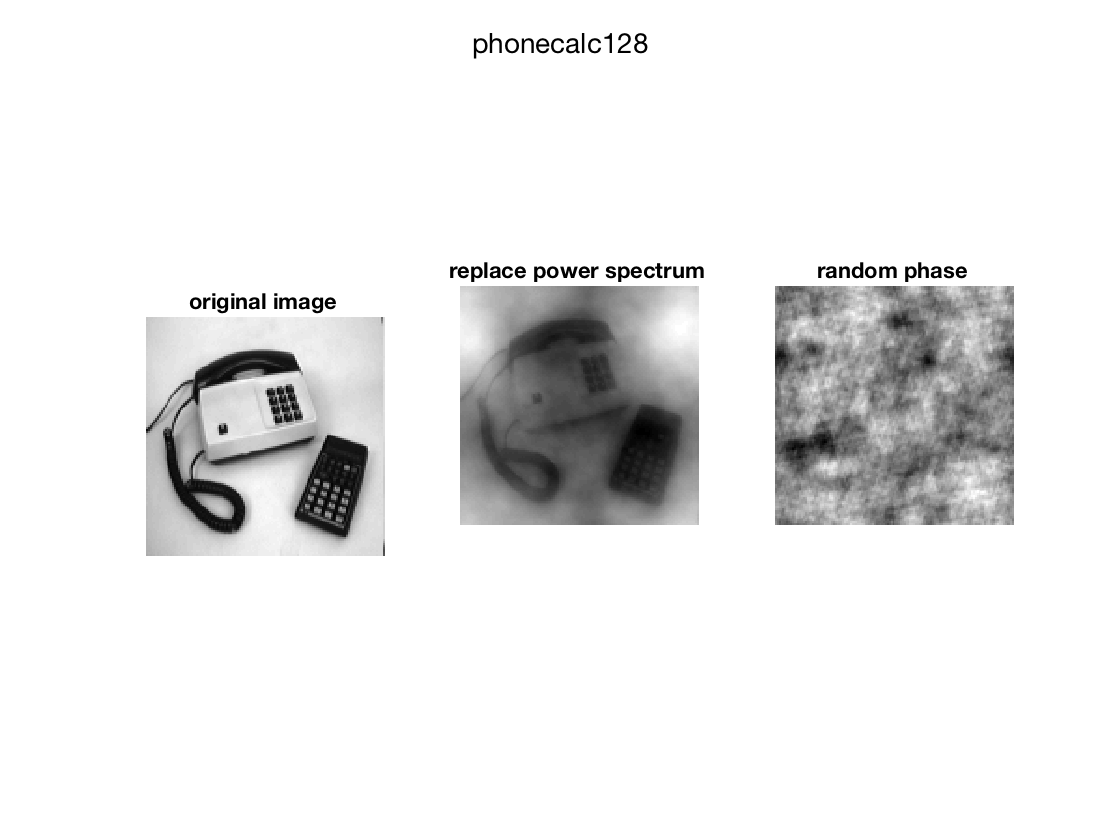
\includegraphics[width=\maxwidth{56.196688409433015em}]{figure_16}
\end{center}
\begin{matlabcode}
figure
%%% few128
subplot(1,3,1);
suptitle('few128')
showgrey(img_2);
title('original image ');
subplot(1,3,2);
showgrey(img_2_p2i);
title('replace power spectrum');
subplot(1,3,3);
showgrey(img_2_rpi);
title('random phase ');
\end{matlabcode}
\begin{center}
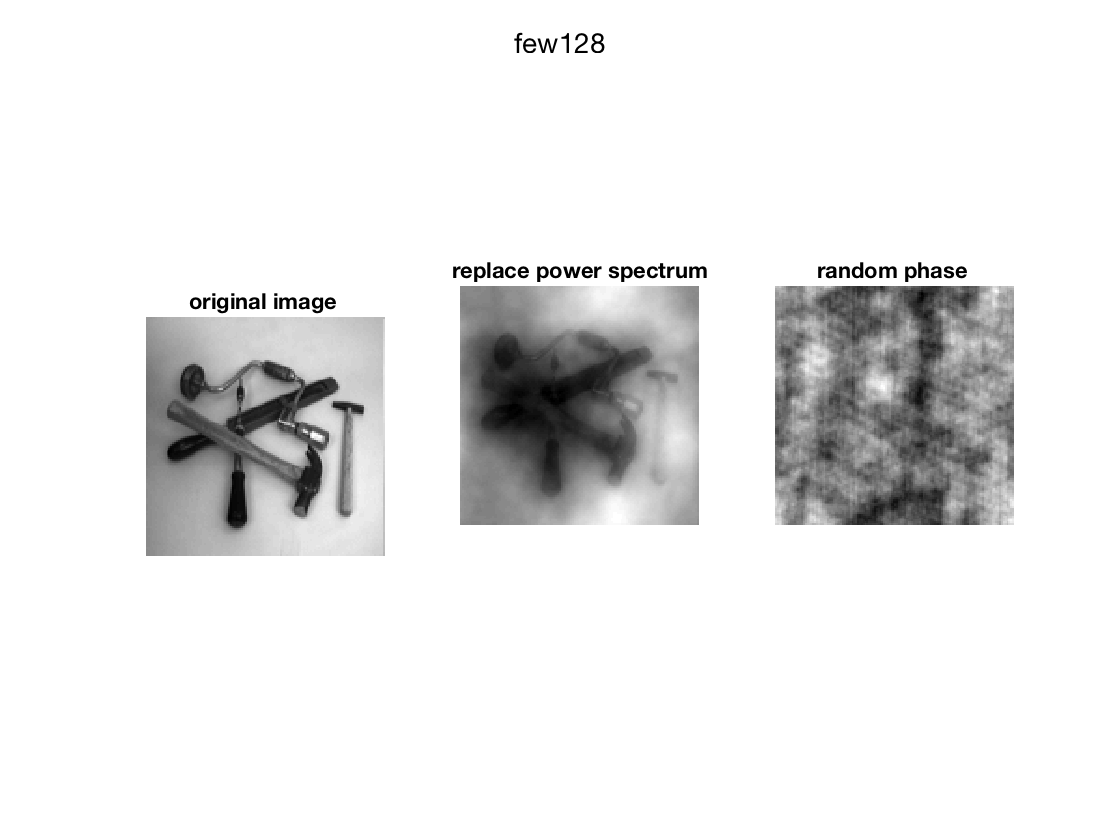
\includegraphics[width=\maxwidth{56.196688409433015em}]{figure_17}
\end{center}
\begin{matlabcode}
figure
%%% nallo128
subplot(1,3,1);
suptitle('nallo128')
showgrey(img_3);
title('original image');
subplot(1,3,2);
showgrey(img_3_p2i);
title('replace power spectrum');
subplot(1,3,3);
showgrey(img_3_rpi);
title('random phase');
\end{matlabcode}
\begin{center}
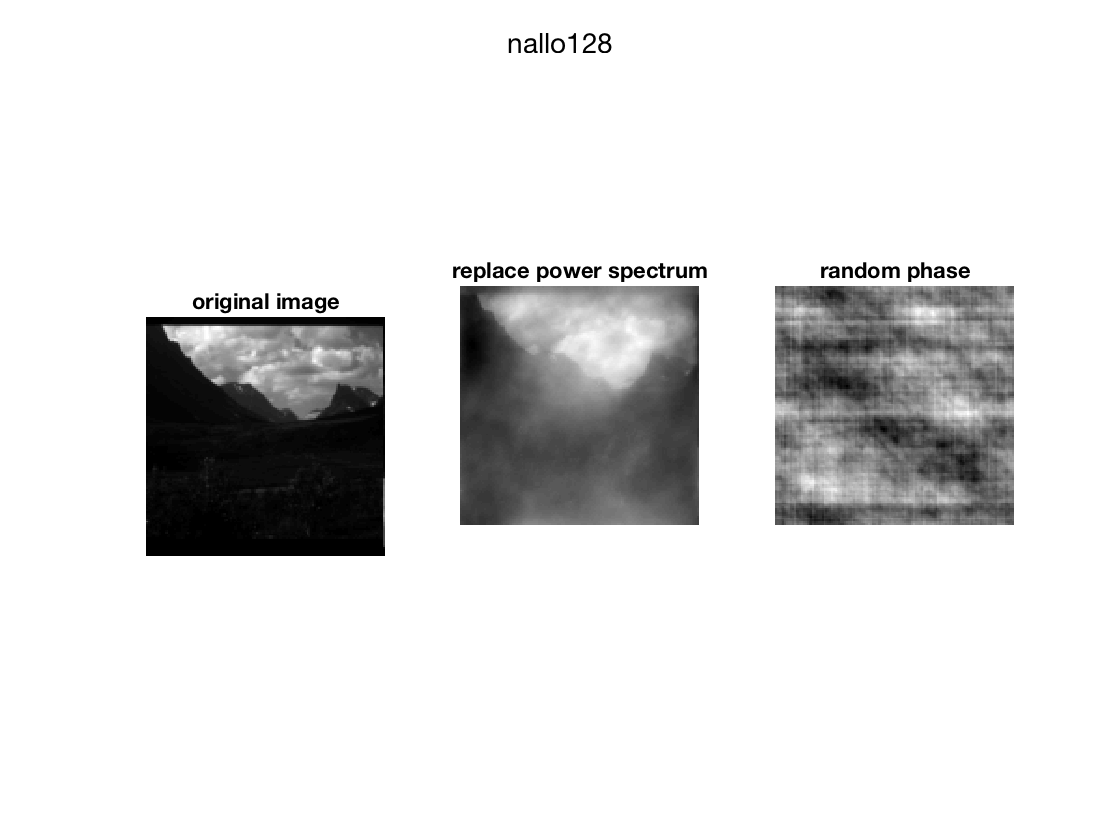
\includegraphics[width=\maxwidth{56.196688409433015em}]{figure_18}
\end{center}

\begin{par}
\begin{flushleft}
\textbf{Answer:}
\end{flushleft}
\end{par}

\begin{par}
\begin{flushleft}
The phase contains the information of edges and shapes in an image while the magnitude contains the information of intensity. So if we change the magnitude while retain the same phase, we can still recognize the objects in one image. On the other hand, if we give a random phase and remain the same magnitude, we can only get an image with some fogs and tell nothing on it.
\end{flushleft}
\end{par}


\begin{par}
\begin{flushleft}
\textbf{Question 14:}
\end{flushleft}
\end{par}

\begin{par}
\begin{flushleft}
Show the impulse response and variance for the above-mentioned t-values. What are the variances of your discretized Gaussian kernel for t = 0.1, 0.3, 1.0, 10.0 and
\end{flushleft}
\end{par}

\begin{par}
\begin{flushleft}
100.0?
\end{flushleft}
\end{par}

\begin{par}
\begin{flushleft}
\textbf{Answer:}
\end{flushleft}
\end{par}

\begin{par}
\begin{flushleft}
The figure shows the impulse response:
\end{flushleft}
\end{par}

\begin{matlabcode}
subplot(1,5,1);
t = 0.1;
psf = gaussfft(deltafcn(128,128),t);
showgrey(psf);
title('t=0.1');
va_01 = variance(psf);
subplot(1,5,2);
t = 0.3;
psf = gaussfft(deltafcn(128,128),t);
showgrey(psf);
title('t=0.3');
va_03 = variance(psf);

subplot(1,5,3);
t = 1.0;
psf = gaussfft(deltafcn(128,128),t);
showgrey(psf);
title('t=1.0');
subplot(1,5,4);
va_10 = variance(psf);

t = 10;
psf = gaussfft(deltafcn(128,128),t);
showgrey(psf);
title('t=10');
va_100 = variance(psf);

subplot(1,5,5);
t = 100;
psf = gaussfft(deltafcn(128,128),t);
showgrey(psf);
title('t=100');
\end{matlabcode}
\begin{center}
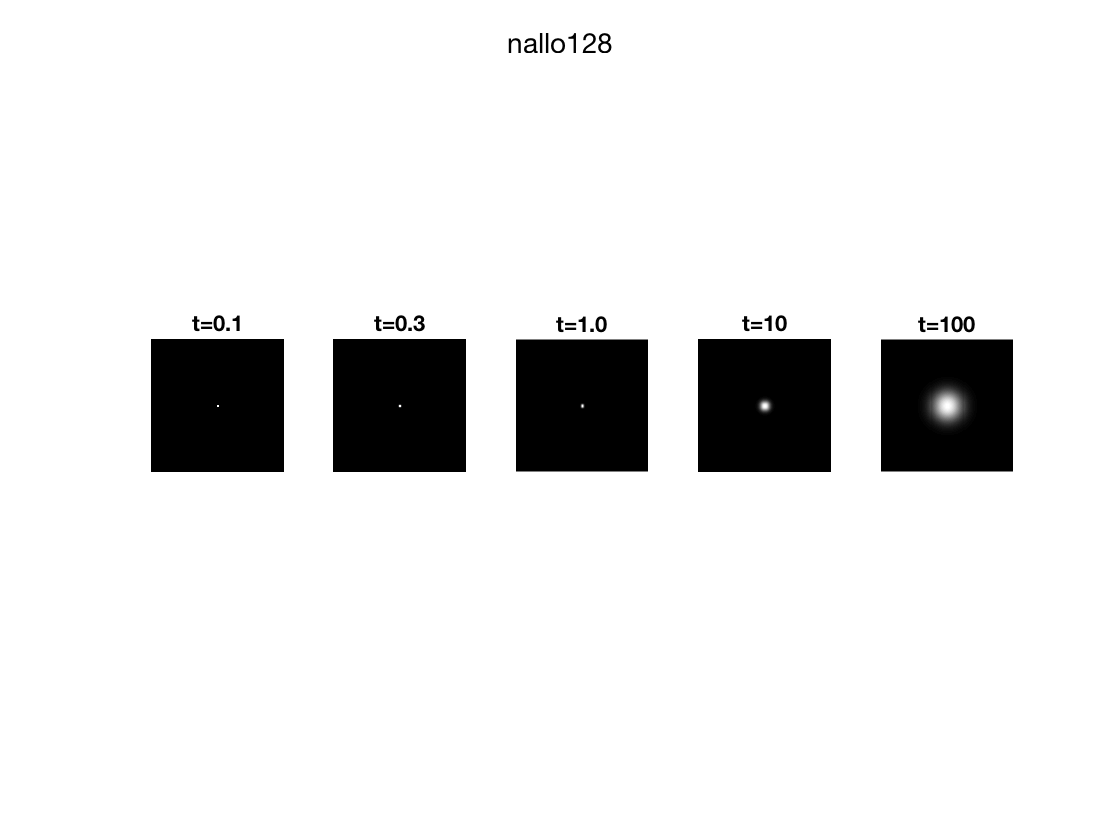
\includegraphics[width=\maxwidth{56.196688409433015em}]{figure_19}
\end{center}
\begin{matlabcode}
va_1000 = variance(psf);
\end{matlabcode}

\begin{par}
\begin{flushleft}
The following table shows the variance;
\end{flushleft}
\end{par}

\begin{matlabcode}
sprintf('t=0.1')
\end{matlabcode}
\begin{matlaboutput}
ans = 't=0.1'
\end{matlaboutput}
\begin{matlabcode}
disp(va_01)
\end{matlabcode}
\begin{matlaboutput}
    0.0133    0.0000
    0.0000    0.0133
\end{matlaboutput}
\begin{matlabcode}
sprintf('t=0.3')
\end{matlabcode}
\begin{matlaboutput}
ans = 't=0.3'
\end{matlaboutput}
\begin{matlabcode}
disp(va_03)
\end{matlabcode}
\begin{matlaboutput}
    0.2811    0.0000
    0.0000    0.2811
\end{matlaboutput}
\begin{matlabcode}
sprintf('t=1')
\end{matlabcode}
\begin{matlaboutput}
ans = 't=1'
\end{matlaboutput}
\begin{matlabcode}
disp(va_10)
\end{matlabcode}
\begin{matlaboutput}
    1.0000    0.0000
    0.0000    1.0000
\end{matlaboutput}
\begin{matlabcode}
sprintf('t=10')
\end{matlabcode}
\begin{matlaboutput}
ans = 't=10'
\end{matlaboutput}
\begin{matlabcode}
disp(va_100)
\end{matlabcode}
\begin{matlaboutput}
   10.0000    0.0000
    0.0000   10.0000
\end{matlaboutput}
\begin{matlabcode}
sprintf('t=100')
\end{matlabcode}
\begin{matlaboutput}
ans = 't=100'
\end{matlaboutput}
\begin{matlabcode}
disp(va_1000)
\end{matlabcode}
\begin{matlaboutput}
  100.0000    0.0000
    0.0000  100.0000
\end{matlaboutput}


\begin{par}
\begin{flushleft}
\_\_\_\_\_\_\_\_\_\_\_\_\_\_\_\_\_\_\_\_\_\_\_\_\_\_\_\_\_\_\_\_\_\_\_\_\_\_\_\_\_\_\_\_\_\_
\end{flushleft}
\end{par}

\begin{par}
\begin{flushleft}
\textbf{Question 15} :
\end{flushleft}
\end{par}

\begin{par}
\begin{flushleft}
Are the results different from or similar to the estimated variance? How does the result correspond to the ideal continuous case? Lead: think of the relation between spatial and Fourier domains for different values of t.
\end{flushleft}
\end{par}

\begin{par}
\begin{flushleft}
\textbf{Answer:}
\end{flushleft}
\end{par}

\begin{par}
\begin{flushleft}
The results are similar to the estimated variance but there is a little difference on it.  when value of t is larger, the difference becomes small. After t \textgreater{}1, the variances are almost the same as the estimated ones.t here is actually the Gaussian filter’s variance. It controls how ‘tight’ the Gaussian would be so if t is larger, the range of smoothness would be larger. if t \textless{} 1 , it means that some of the information on this pixel will lose, therefore the variance will be different.
\end{flushleft}
\end{par}


\begin{par}
\begin{flushleft}
\_\_\_\_\_\_\_\_\_\_\_\_\_\_\_\_\_\_\_\_\_\_\_\_\_\_\_\_\_\_\_\_\_\_\_\_\_\_\_\_\_\_\_\_\_\_
\end{flushleft}
\end{par}

\begin{par}
\begin{flushleft}
\textbf{Question 16:}
\end{flushleft}
\end{par}

\begin{par}
\begin{flushleft}
Convolve a couple of images with Gaussian functions of different variances (like t = 1.0, 4.0, 16.0, 64.0 and 256.0) and present your results. What effects can you observe?
\end{flushleft}
\end{par}

\begin{par}
\begin{flushleft}
\textbf{Answer:}
\end{flushleft}
\end{par}

\begin{par}
\begin{flushleft}
When our t is bigger, the much vaguer the image we would have. Which means we have much more smoothing figures.
\end{flushleft}
\end{par}

\begin{par}
\begin{flushleft}
Here are 3 example images with different variances:
\end{flushleft}
\end{par}

\begin{matlabcode}
%%% first image: phonecalc128
figure
subplot(3,2,1);
showgrey(img_1);
title('phonecal128');
subplot(3,2,2);
t = 1;
psf = gaussfft(img_1,t);
showgrey(psf);
title('t=1');
subplot(3,2,3);
t = 4;
psf = gaussfft(img_1,t);
showgrey(psf);
title('t=4');
subplot(3,2,4);
t = 16;
psf = gaussfft(img_1,t);
showgrey(psf);
title('t=4');
subplot(3,2,5);
t = 64;
psf = gaussfft(img_1,t);
showgrey(psf);
title('t=64');
subplot(3,2,6);
t = 256;
psf = gaussfft(img_1,t);
showgrey(psf);
title('t=256');
\end{matlabcode}
\begin{center}
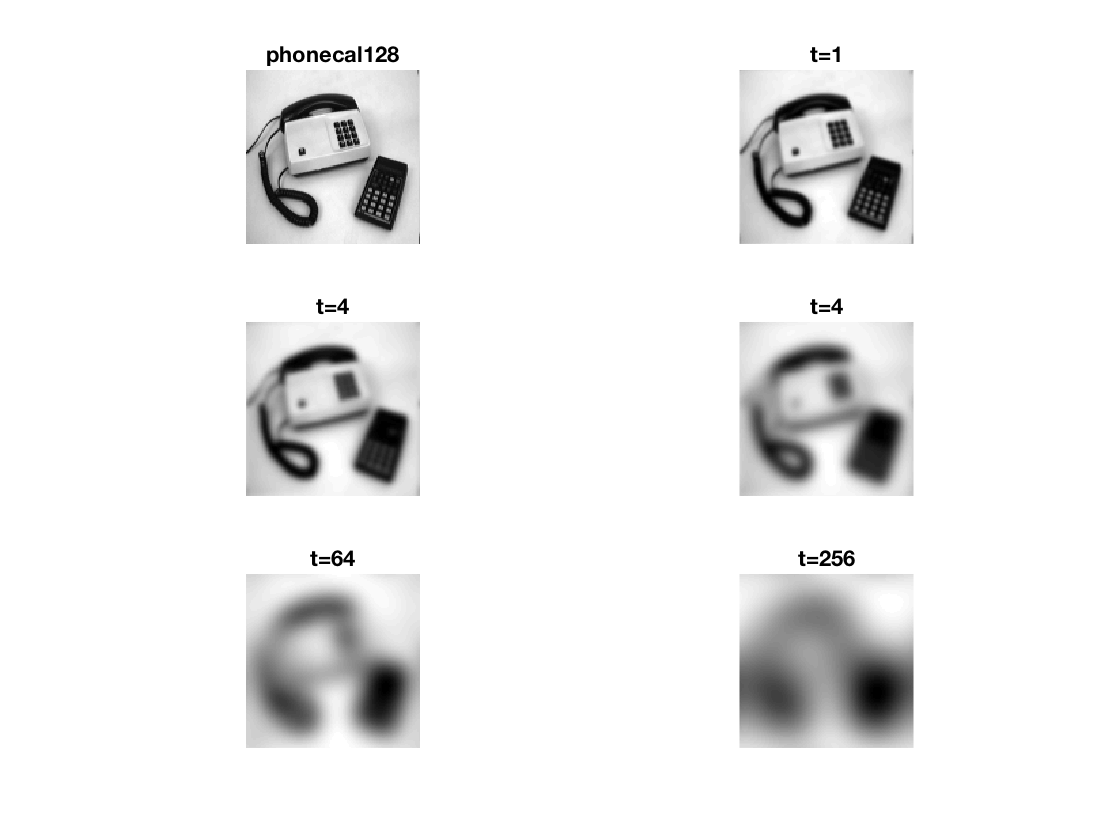
\includegraphics[width=\maxwidth{56.196688409433015em}]{figure_20}
\end{center}
\begin{matlabcode}
%%%% second image : few128
figure
subplot(3,2,1);
showgrey(img_2);
title('phonecalc128');
subplot(3,2,2);
t = 1;
psf = gaussfft(img_2,t);
showgrey(psf);
title('t=1');
subplot(3,2,3);
t = 4;
psf = gaussfft(img_2,t);
showgrey(psf);
title('t=4');
subplot(3,2,4);
t = 16;
psf = gaussfft(img_2,t);
showgrey(psf);
title('t=4');
subplot(3,2,5);
t = 64;
psf = gaussfft(img_2,t);
showgrey(psf);
title('t=64');
subplot(3,2,6);
t = 256;
psf = gaussfft(img_2,t);
showgrey(psf);
title('t=256');
\end{matlabcode}
\begin{center}
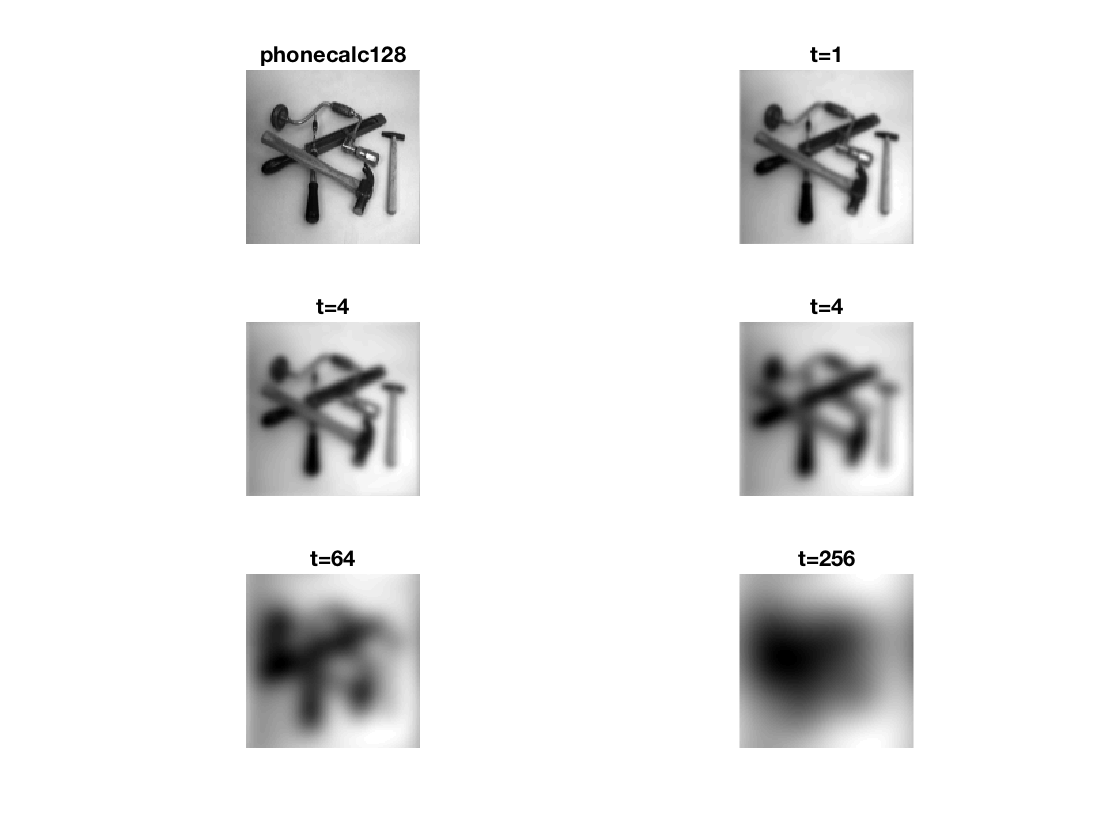
\includegraphics[width=\maxwidth{56.196688409433015em}]{figure_21}
\end{center}
\begin{matlabcode}
%%% third image: nallo128
figure
subplot(3,2,1);
showgrey(img_3);
title('nallo128');
subplot(3,2,2);
t = 1;
psf = gaussfft(img_3,t);
showgrey(psf);
title('t=1');
subplot(3,2,3);
t = 4;
psf = gaussfft(img_3,t);
showgrey(psf);
title('t=4');
subplot(3,2,4);
t = 16;
psf = gaussfft(img_3,t);
showgrey(psf);
title('t=4');
subplot(3,2,5);
t = 64;
psf = gaussfft(img_3,t);
showgrey(psf);
title('t=64');
subplot(3,2,6);
t = 256;
psf = gaussfft(img_3,t);
showgrey(psf);
title('t=256');
\end{matlabcode}
\begin{center}
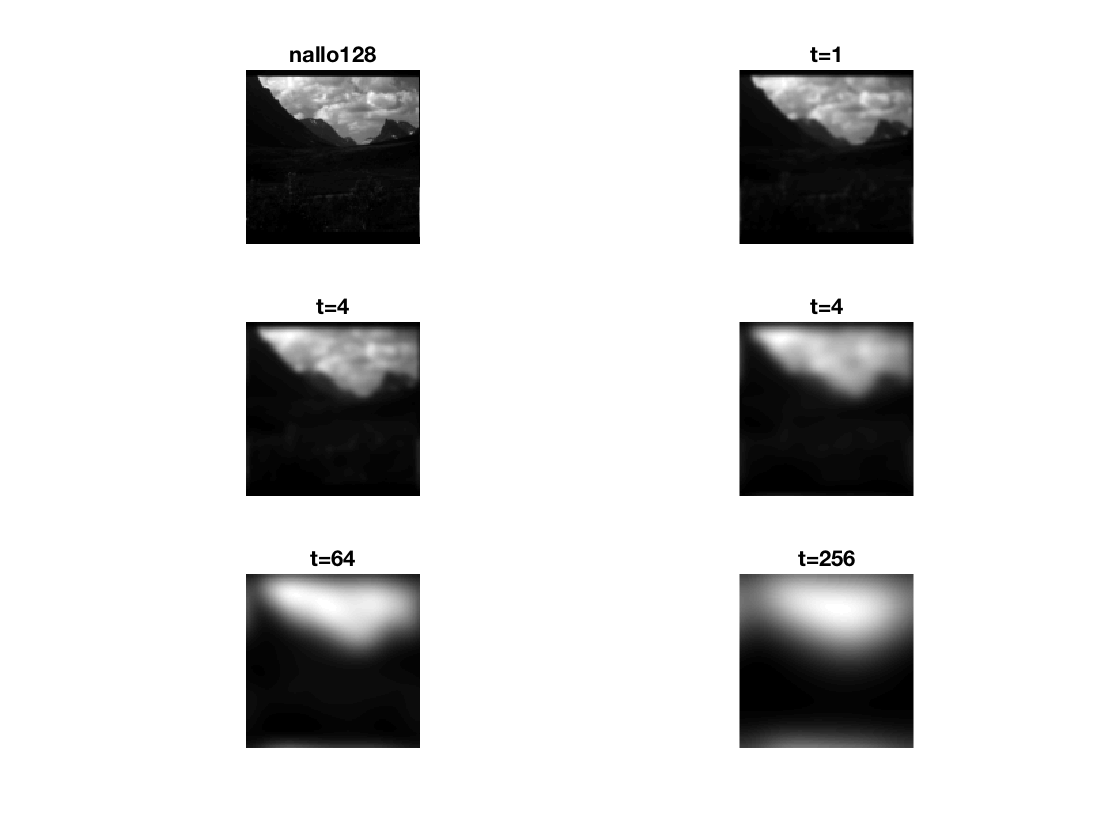
\includegraphics[width=\maxwidth{56.196688409433015em}]{figure_22}
\end{center}


\begin{par}
\begin{flushleft}
\textbf{Question 17:}
\end{flushleft}
\end{par}

\begin{par}
\begin{flushleft}
What are the positive and negative effects for each type of filter? Describe what you observe and name the effects that you recognize. How do the results depend on the filter parameters? Illustrate with Matlab figure(s)
\end{flushleft}
\end{par}

\begin{par}
\begin{flushleft}
\textbf{Answer:}
\end{flushleft}
\end{par}

\begin{par}
\begin{flushleft}
The origin image with Gaussian noise and salt-and-pepper noise is shown below:
\end{flushleft}
\end{par}

\begin{matlabcode}
office = office256;
add = gaussnoise(office,16);
sap = sapnoise(office,0.1,256);
figure
subplot(1,3,1);
showgrey(office);
title('origin');
subplot(1,3,2);
showgrey(add);
title('add');
subplot(1,3,3);
showgrey(sap);
title('sap');
\end{matlabcode}
\begin{center}
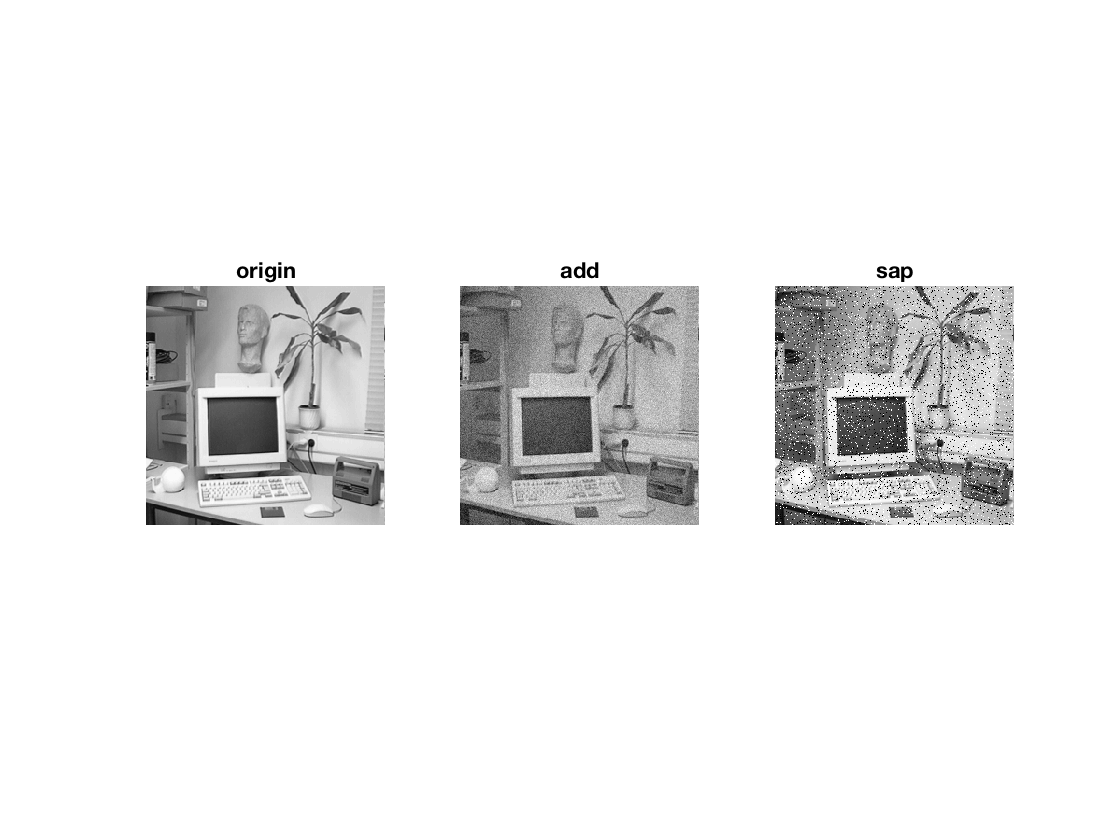
\includegraphics[width=\maxwidth{56.196688409433015em}]{figure_23}
\end{center}

\begin{par}
\begin{flushleft}
For Gaussian filter:
\end{flushleft}
\end{par}

\begin{par}
\begin{flushleft}
      It cannot remove the salt-and-pepper noise well, but for the Gaussian noise, it works better. However, if we set the variance too large, then the image become blur. Therefore, with Gaussian Filter, I set the variance 2 only.
\end{flushleft}
\end{par}

\begin{matlabcode}
%%%% 1. Gaussian Smoothing
gauadd = gaussfft(add,2);
gausap = gaussfft(sap,2);
figure
subplot(2,1,1);
showgrey(gauadd);
title('gaussian filter with gaussian noise');
subplot(2,1,2);
showgrey(gausap);
%showgrey(gausap);
title('gaussian filter with sap noise');
\end{matlabcode}
\begin{center}
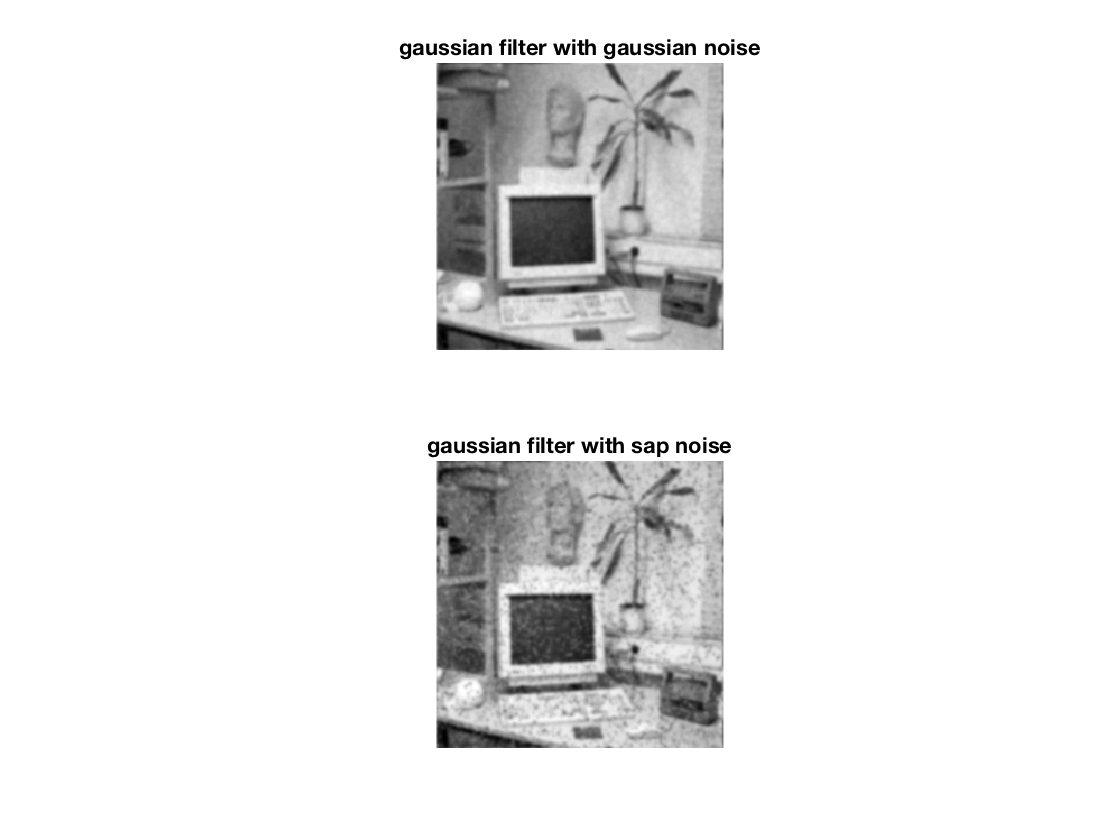
\includegraphics[width=\maxwidth{56.196688409433015em}]{figure_24}
\end{center}

\begin{par}
\begin{flushleft}
For Median filter:
\end{flushleft}
\end{par}

\begin{par}
\begin{flushleft}
            It removes the salt-and-pepper noise well, but for the Gaussian noise, the result with median filter is not as good as Gaussian filter, but it is just ok. It is because median filter eliminates the local extreme value. It creates a paint-like image and the larger the window height and width we set, the more paint-like image we receive. So with the Median filter, I set the (height, width) = (3,3)
\end{flushleft}
\end{par}

\begin{matlabcode}
%%%% 2.median filter
medadd = medfilt(add,3,3);
medsap = medfilt(sap,3,3);
figure
subplot(2,1,1);
showgrey(medadd);
title('median filter with gaussian noise');
subplot(2,1,2);
showgrey(medsap);
title('median filter with sap noise');
\end{matlabcode}
\begin{center}
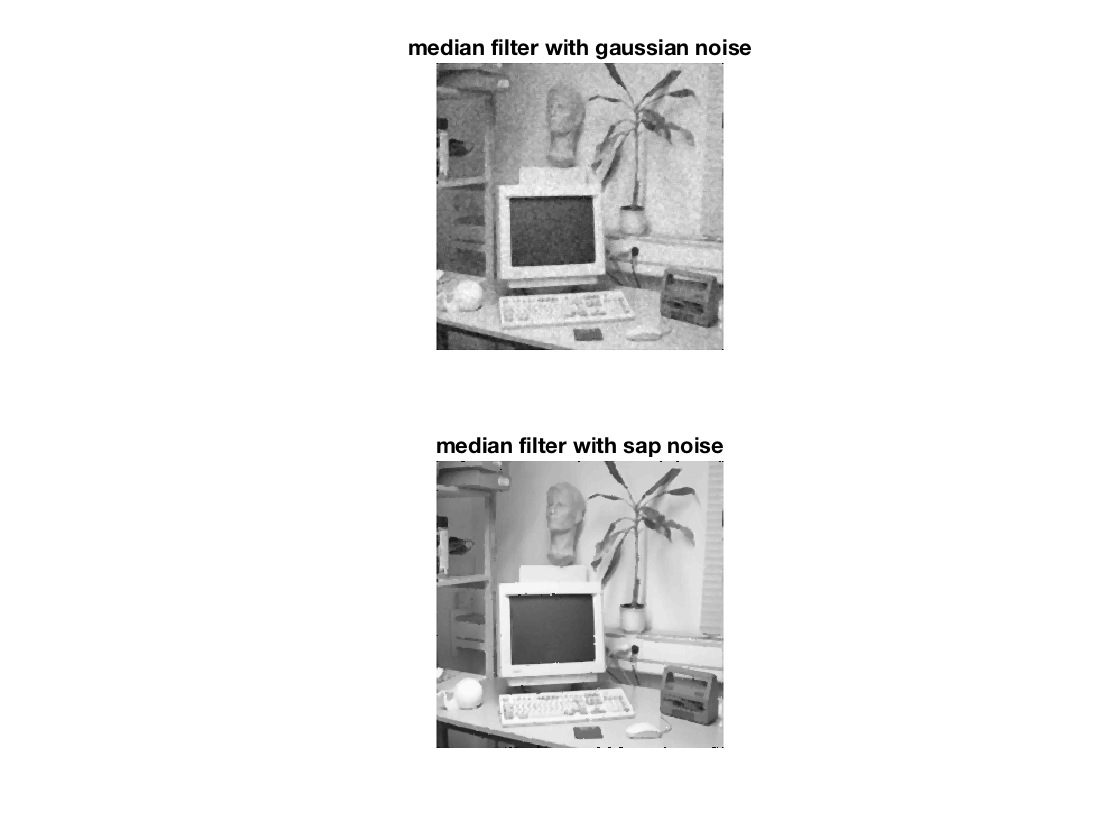
\includegraphics[width=\maxwidth{56.196688409433015em}]{figure_25}
\end{center}

\begin{par}
\begin{flushleft}
For low pass filter:
\end{flushleft}
\end{par}

\begin{par}
\begin{flushleft}
It also removes the salt-and-pepper noise but the result is not as good as the median filter. The result of the image with salt-and-pepper noise is similar with the image with Gaussian noise. 
\end{flushleft}
\end{par}

\begin{matlabcode}
lopasadd = ideal(add,0.3,'l');
lopassap = ideal(add,0.3,'l');
figure
subplot(2,1,1);
showgrey(lopasadd);
title('low pass filter with gaussian noise');
subplot(2,1,2);
showgrey(lopassap);
title('low pass filter with sap noise');
\end{matlabcode}
\begin{center}
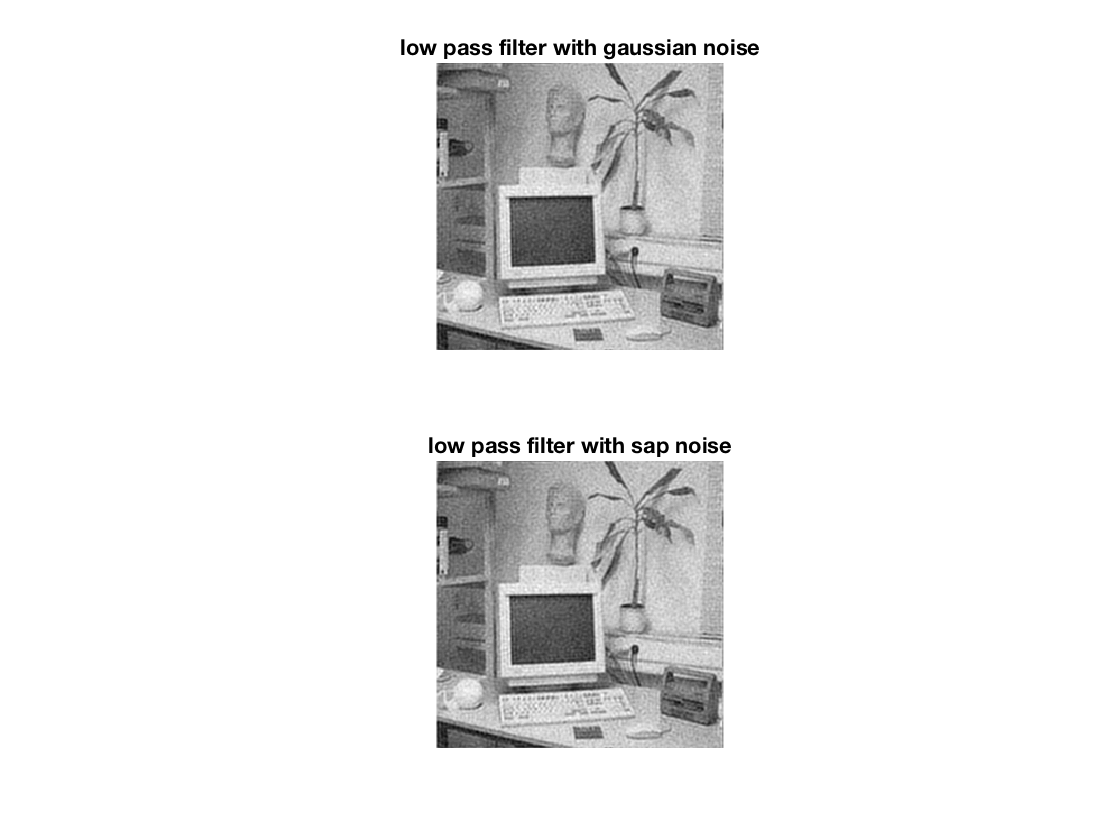
\includegraphics[width=\maxwidth{56.196688409433015em}]{figure_26}
\end{center}


\begin{par}
\begin{flushleft}
\_\_\_\_\_\_\_\_\_\_\_\_\_\_\_\_\_\_\_\_\_\_\_\_\_\_\_\_\_\_\_\_\_\_\_\_\_\_\_\_\_\_\_\_\_\_
\end{flushleft}
\end{par}

\begin{par}
\begin{flushleft}
\textbf{Question 18 }:
\end{flushleft}
\end{par}

\begin{par}
\begin{flushleft}
What conclusions can you draw from comparing the results of the respective methods? 
\end{flushleft}
\end{par}

\begin{par}
\begin{flushleft}
\textbf{Answer}:
\end{flushleft}
\end{par}

\begin{par}
\begin{flushleft}
If we have an image with salt-and-pepper noise, we can use Medium filter to enhance the quality of image Because it will remove the local maximum value. If we want to remove Gaussian noise to improve the quality, we can use Gaussian filter.
\end{flushleft}
\end{par}


\begin{par}
\begin{flushleft}
\_\_\_\_\_\_\_\_\_\_\_\_\_\_\_\_\_\_\_\_\_\_\_\_\_\_\_\_\_\_\_\_\_\_\_\_\_\_\_\_\_\_\_\_\_\_
\end{flushleft}
\end{par}

\begin{par}
\begin{flushleft}
\textbf{Question 19} :
\end{flushleft}
\end{par}

\begin{par}
\begin{flushleft}
What effects do you observe when subsampling the original image and the smoothed variants? Illustrate both filters with the best results found for iteration i = 4.
\end{flushleft}
\end{par}

\begin{par}
\begin{flushleft}
\textbf{Answer:}
\end{flushleft}
\end{par}

\begin{par}
\begin{flushleft}
When subsampling the original image, we can see that the details of the image are gradually removed. For example, in the original image, we can see clearly the keyboard of telephone, after subsampling or smoothed variants, we can only see a large black rectangle there. On the other hand, the edge of the object becomes rough and we can see the blocks with larger and larger different level of grey on the edge.
\end{flushleft}
\end{par}

\begin{par}
\begin{flushleft}
Comparing to the image subsampled only and the image which is smoothed before subsampling, we can found that the image that is smoothed before subsampled has much pleasing edge. On the other hand, compare to the image smoothed with Gaussian filter, the image with low pass filter retain more details and looks less smoothed if we want to remain much sharp edge while the image smoothed with Gaussian filter is more smoothed with sharper edge.
\end{flushleft}
\end{par}

\begin{par}
\begin{flushleft}
            The following figures shows the comparison between smoothed before subsampling and only subsampling and the images with two filters before subsampling:
\end{flushleft}
\end{par}

\begin{par}
\begin{flushleft}
 
\end{flushleft}
\end{par}

\begin{par}
\begin{flushleft}
Gaussian filter before subsampling:
\end{flushleft}
\end{par}

\begin{matlabcode}
img = phonecalc256;
smoothing = img;
N = 4;
figure
suptitle('gaussian filter and subsampling');
for i=1:N
    if i>1
        img = rawsubsample(img);
        smoothing = gaussfft(smoothing,0.7);
        smoothing = rawsubsample(smoothing);
    end
    subplot(2,N,i)
    showgrey(img)
    title(['n = ',num2str(i),' subsampling']);
    subplot(2,N,i+N)
    showgrey(smoothing)
    title(['n = ',num2str(i), ' with smoothing']);
end
\end{matlabcode}
\begin{center}
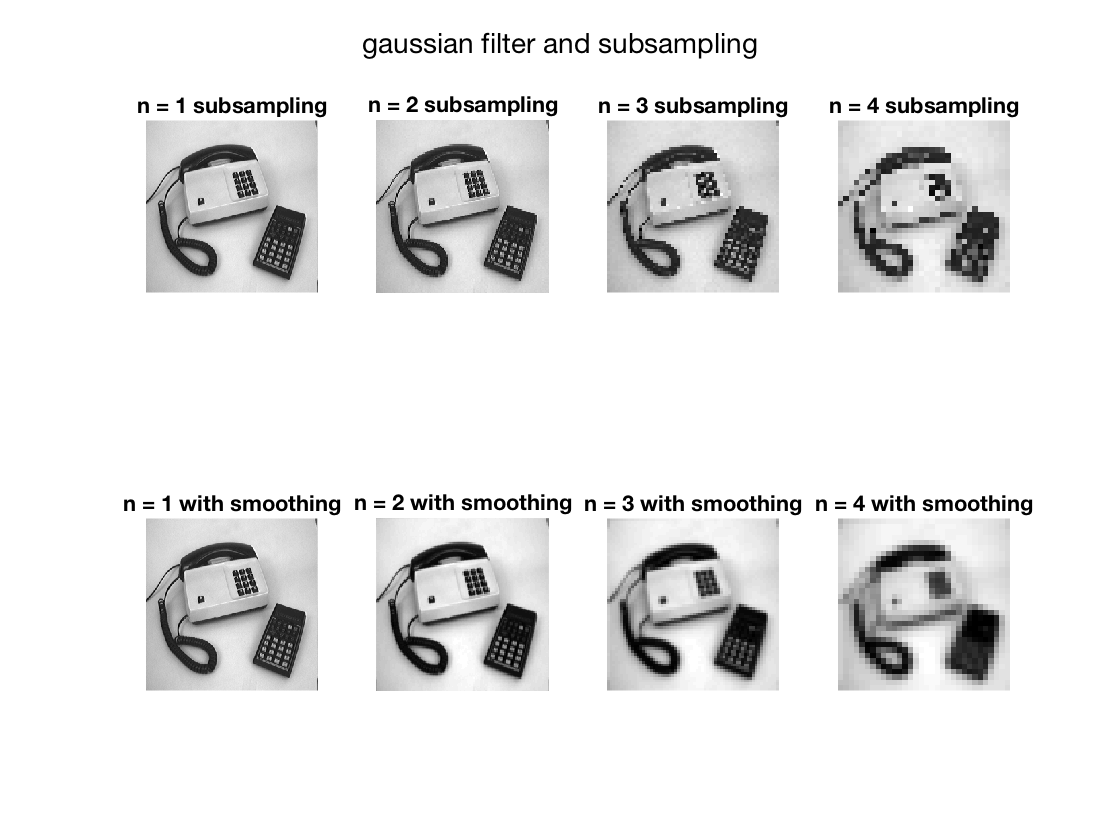
\includegraphics[width=\maxwidth{56.196688409433015em}]{figure_27}
\end{center}

\begin{par}
\begin{flushleft}
                    (with the variance of Gaussian is 0.7)
\end{flushleft}
\end{par}

\begin{par}
\begin{flushleft}
Low pass filter before subsampling:
\end{flushleft}
\end{par}

\begin{matlabcode}
img = phonecalc256;
smoothing = img;
N = 4;
figure
suptitle('low pass filter and subsampling');
for i=1:N
    if i>1
        img = rawsubsample(img);
        smoothing = ideal(smoothing,0.3,'l');
        smoothing = rawsubsample(smoothing);
    end
 
    subplot(2,N,i)
    showgrey(img)
    title(['n = ',num2str(i),' subsampling']);
    subplot(2,N,i+N)
    showgrey(smoothing)
    title(['n = ',num2str(i), ' with smoothing']);
end
\end{matlabcode}
\begin{center}
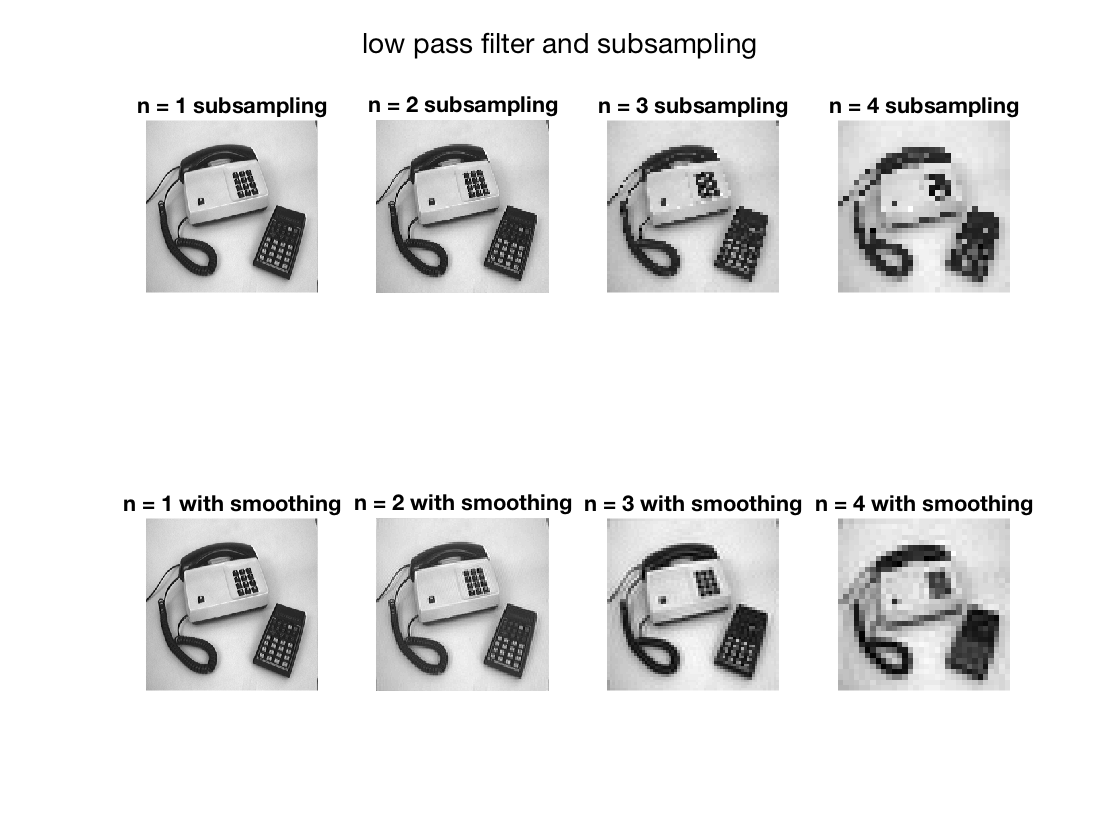
\includegraphics[width=\maxwidth{56.196688409433015em}]{figure_28}
\end{center}
\begin{matlabcode}
    
\end{matlabcode}


\begin{par}
\begin{flushleft}
\_\_\_\_\_\_\_\_\_\_\_\_\_\_\_\_\_\_\_\_\_\_\_\_\_\_\_\_\_\_\_\_\_\_\_\_\_\_\_\_\_\_\_\_\_\_
\end{flushleft}
\end{par}

\begin{par}
\begin{flushleft}
\textbf{Question 20:}
\end{flushleft}
\end{par}

\begin{par}
\begin{flushleft}
What conclusions can you draw regarding the effects of smoothing when combined with subsampling? Hint: think in terms of frequencies and side effects.
\end{flushleft}
\end{par}

\begin{par}
\begin{flushleft}
\textbf{Answer:}
\end{flushleft}
\end{par}

\begin{par}
\begin{flushleft}
If we want to decrease the resolution of one image while maintaining its quality, it is better to use low pass filter first to smooth and then do the subsampling process. The implemented image would look much more pleasing than we do subsample only. The reason is that , when we do the subsampling, we cut off the higher frequency in the image, so the information in higher frequency goes to lower frequency and causes the disappear of fine structure and distort the coarser structure, which is called aliasing. If we decrease the highest frequency before sampling by blurring the image,then we can prevent the aliasing.
\end{flushleft}
\end{par}


\begin{matlabcode}
function revpic = gaussfft(pic,t)
picHat = fft2(pic);
[x,y] = size(picHat);
x1 = 0:x-1;
y1 = 0:y-1;
[x1g,x2g] = meshgrid(x1,y1);
x1g = fftshift(x1g,2);
x2g = fftshift(x2g,1);
gau = (1/(2*pi*t)) * exp(-((x1g - x/2).^2 + (x2g - y/2).^2)/(t*2));
gauHat = fft2(gau);

gxpic = gauHat .* picHat;
revpic = real(ifft2(gxpic));
end

function fftwave(u, v, sz)
  if (nargin <= 0) 
    error('Requires at least two input arguments.') 
  end
  if (nargin == 2) 
    sz = 128; 
  end
  
  Fhat = zeros(sz);
  Fhat(u, v) = 1;
  
  F = ifft2(Fhat);
  Fabsmax = max(abs(F(:)));
  
  subplot(3, 2, 1);
  showgrey(Fhat);
  title(sprintf('Fhat: (u, v) = (%d, %d)', u, v))
  
  % What is done by these instructions?
  if (u <= sz/2)
    uc = u - 1;
  else
    uc = u - 1 - sz;
  end
  if (v <= sz/2)
    vc = v - 1;
  else
    vc = v - 1 - sz;
  end
  
  wavelength = 1/sqrt(1/abs(uc-1)^2+1/abs(vc-1)^2);  % Replace by correct expression 
  amplitude = 1/(128);   % Replace by correct expression

  subplot(3, 2, 2);
  showgrey(fftshift(Fhat));
  title(sprintf('centered Fhat: (uc, vc) = (%d, %d)', uc, vc))
  %disp(uc)
  subplot(3, 2, 3);
  showgrey(real(F), 64, -Fabsmax, Fabsmax);
  title('real(F)')
  
  subplot(3, 2, 4);
  showgrey(imag(F), 64, -Fabsmax, Fabsmax);
  title('imag(F)')
  
  subplot(3, 2, 5);
  showgrey(abs(F), 64, -Fabsmax, Fabsmax);
  title(sprintf('abs(F) (amplitude %f)', amplitude))
  
  subplot(3, 2, 6);
  showgrey(angle(F), 64, -pi, pi);
  title(sprintf('angle(F) (wavelength %f)', wavelength))
  end
 
\end{matlabcode}

\end{document}
